\chapter{Task-driven Assessment of Dimensionality Reduction Methods for Machine Learning and Black-Box Optimisation}\label{ch:ch04:dim_red}

\section{Introduction}
\label{sec:ch04:intro}
High-dimensional data is ubiquitous in numerous application domains of machine learning and black-box optimisation.


In areas ranging from computer vision~\citep{SchEtAl15}, genome sequencing~\citep{VanEtAl22} and anomaly detection~\citep{TalEtAl21} to engineering~\citep{PreEtAl24}, hyperparameter optimisation~\citep{SehEtAl22} and neural architecture search~\citep{ElsEtAl19}, complex datasets with a large number of features defining 

a space to be searched for desirable design choices or solutions 
need to be handled effectively, in order to ensure that machine learning and  black-box optimisation algorithms applied to them are as accurate, efficient and scalable as possible. 
This poses a fundamental challenge in many applications, due to the curse of dimensionality, where the volume of the search space grows exponentially as data dimensionality increases, thereby degrading the performance of an algorithm applied to that data.
Data points become sparser in high dimensions, making it difficult for a machine learning algorithm to capture the underlying structure of the data and for a  black-box optimisation algorithm to locate good solutions for a given problem. 
At the same time, computational complexity severely increases, as well as the risk of overfitting in machine learning applications, leading to poor generalisation ability.

Dimensionality reduction methods serve as a crucial tool to address the challenge of manipulating high-dimensional data by evaluating the available information and extracting essential features from it.

The core principle of dimensionality reduction is to transform data from a high-dimensional space to a lower-dimensional one, revealing the underlying 

structure that is concealed in the original

data. 

Operating in a low-dimensional space enables machine learning algorithms to capture meaningful patterns in the data and  black-box optimisation algorithms to search for an optimal solution more effectively.
Traditionally, dimensionality reduction is used for machine learning tasks to reduce the input size of the data, as many machine learning algorithms (such as random forests~\citep{Breiman01} and support vector machines~\citep{CorVap95}) scale poorly with the number of features 

in terms of computational complexity. 
Dimensionality reduction methods are also employed for data clustering and visualisation~\citep{VanHin08}.
For classical applications, good performance of machine learning algorithms heavily relies on the ability of dimensionality reduction methods to preserve essential 

information contained in the data.
In the context of machine learning, this leads to higher interpretability of the models, reduced 

time and space complexity, less overfitting, and ultimately improved generalisation performance of machine learning models~\citep{JiaEtAl22}.

The curse of dimensionality is also a major obstacle for solving optimisation problems~\citep{Garnett23}. 

High-dimensional optimisation problems are widely encountered in the field of machine learning; for instance, the performance of machine learning algorithms crucially depends on the chosen values of the hyperparameters that govern their behaviour, and the performance of neural networks on some task of interest is heavily impacted by the choice of its architectural components~\cite{ElsEtAl19}.
Finding a well-performing set of hyperparameter values or a well-suited neural architecture for a given problem are  black-box optimisation problems, typically high-dimensional and expensive to evaluate.


Black-box optimisation algorithms used to tackle problems like these




do not have access to any information about the problem instance they aim to solve other than the evaluated samples from the search space. 

Typically, as the dimensionality of the search space increases, the volume grows exponentially, making it progressively more challenging for these algorithms to effectively locate good solutions. They also take more time to run in high-dimensional spaces.

In this context, dimensionality reduction methods have the potential to facilitate the optimisation process by transforming the high-dimensional problem landscape into a lower-dimensional one that may well be easier to tackle. 
We argue that preserving essential information about the data might not be imperative in the context of  black-box optimisation tasks (at least not in the way required for machine learning) if the performance of the optimisation algorithm is enhanced by navigating a more tractable landscape (assuming we are able to adequately reconstruct in the original space the points corresponding to the high-quality solutions 


in the reduced space).  

In recent years, there have been some attempts to leverage the power of dimensionality reduction for solving challenging optimisation problems in domains other than hyperparameter optimisation and neural architecture search~\citep{RapEtAl20,AntEtAl22,MeiWan21b,WanEtAl16b,KapEtAl16,AbbEtAl20}, where notably, the performance of (surrogate- and population-based) optimisation algorithms have been boosted by incorporating dimensionality reduction methods into the optimisation process.
Many real-world optimisation applications have high dimensionality, for example, in mechanical engineering~\citep{Jones08} and control problems~\citep{ZuoEtAl24}. 
Likewise, improving machine learning models in terms of scalability and accuracy by means of dimensionality reduction facilitates meta-learning and meta-optimisation approaches, such as algorithm selection and configuration, where state-of-the-art methods typically rely on predictions obtained from machine learning models, \emph{e.g.,} in the context of algorithm configuration~\citep{HutEtAl11}.




Most dimensionality reduction methods are traditionally developed and studied for classical machine learning use-cases.
How they perform in the context of  black-box optimisation is much less understood, despite the close link of the two fields via the existence of problems whose optimisation is crucial for the good performance of machine learning models.


Motivated by these ideas, we perform four complementary task-driven reduction benchmarking analyses, two in the context of machine learning and two in the context of  black-box optimisation, to better understand the strengths and weaknesses of dimensionality reduction methods in these scenarios.
We consider the following tasks:
(1) data clustering (unsupervised machine learning task), (2) classification of tabular data (supervised machine learning task), 
(3) regression for black-box function approximation (using a surrogate model trained on sampled data), 
and (4) a black-box optimisation procedure. 







\textbf{Our contribution:} We conduct a comprehensive benchmarking study on the effectiveness of various dimensionality reduction methods across two machine learning and two black-box optimisation tasks:\\






    \textbf{[Machine learning task 1]} 

    Cluster preservation by assessing the clustering ability in the reduced space, \emph{i.e.,} structural preservation of the data;
    we use hierarchical density-based clustering, which allows for the creation of clusters of varying densities and is 

    robust to parameter selection.\\ 


    \textbf{[Machine learning task 2]} 

    Predictive accuracy of ML algorithms on classification tasks of tabular data in the reduced space, \emph{i.e.,} investigating the effect of reducing the dimensionality of the datasets on the predictive performance of tabular classification models. \\
    \textbf{[Black-box optimisation task 1]}
    Target function approximation via a surrogate model

    in the reduced space, specifically fitting and evaluating the accuracy of a single-target regression random forest model on given benchmark problems, \emph{i.e.,} we predict the function values from the sampled solution candidates for each problem after dimensionality reduction.\\
    \textbf{[Black-box optimisation task 2]} Evaluation of optimiser performance in terms of regret, \emph{i.e.,} distance to the optimum, in the reduced space; as a case study, we focus on a Bayesian optimisation algorithm~\citep{Mockus12,Garnett23}, wherein we carry out the most resource-intensive tasks in the lower-dimensional space.

    This includes Gaussian process regression model training and the definition and evaluation of the acquisition function to predict new solution candidates for subsequent evaluation.






We evaluate the 

efficacy of the dimensionality reduction methods on these tasks on a wide variety of synthetic and real-world benchmarks of varying dimensionality (going as high as several thousand dimensions)
We vary the number of initial samples on which the dimensionality reduction methods are trained, with a particular focus on low sample sizes, which is a common setting in sample-efficient black-box applications.
We also consider multiple target dimensionalities for the reduced space.



From our results, we observed overall considerable differences in the performance of the dimensionality reduction methods we studied across various tasks, initial sample sizes and dimensionalities (both original and reduced).
In particular, the results indicated that, while the benchmarked dimensionality reduction methods exhibit relatively similar performances for the classical machine learning tasks, this does not hold for black-box optimisation scenarios.
In the context of black-box optimisation, depending on the setting at hand, we observed strong performance complementarity between the dimensionality reduction methods, emphasising the need for a careful selection of the dimensionality reduction method with respect to its intended use.

Therefore, our analysis aims to provide insights into how these methods leverage their working mechanisms depending on the task at hand, highlighting the crucial need for a thorough understanding of the intended use of the reduced space before choosing the appropriate method.

The remainder of this paper is organised as follows: in \cref{sec:ch04:dim_red}, we give an overview of dimensionality reduction, position our study in the broader related work context, introduce the methods selected for benchmarking, and give details on the transformation scheme required for dimensionality reduction methods to operate in the context of optimisation.
In \cref{sec:ch04:tasks}, we outline our methodology and present the four tasks designed to assess the performance of dimensionality reduction methods.
In \cref{sec:ch04:exp_setup}, we introduce the benchmark problem suites used in our empirical investigation and provide details on the setup of the experiments.
We present our results in \cref{sec:ch04:res}, analyse the running times of dimensionality reduction methods in \cref{sec:ch04:rt}, critically discuss our findings in \cref{sec:ch04:disc}, and provide concluding remarks in \cref{sec:ch04:concl}.

\section{Dimensionality reduction}
\label{sec:ch04:dim_red}


This section provides the necessary background of the concept of dimensionality reduction, including related work, descriptions of methods selected for this study, and the transformation scheme used for the optimisation tasks.


\subsection{Definition}






    












        


















    





There are two main ways to perform dimensionality reduction, either via feature selection or via feature extraction methods. 
Feature selection involves choosing a subset of features relevant for model construction, while eliminating irrelevant, redundant, and noisy features \citep{TheBho24}.

The goal is to attain the best-performing subset of the original features without resorting to any data transformation.



Despite being the most straightforward way to reduce dimensionality,
a prerequisite for feature selection is that the data exhibits a lower intrinsic dimensionality, allowing for the removal of features with minimal information loss. 
For many problems, this is not the case, as numerous features demonstrate high correlation, and this necessitates that data undergoes some transformation before we can perform dimensionality reduction.

Feature extraction involves creating new features from the original ones, where the new features are essentially images of the old ones through either linear or non-linear mappings \citep{ElhEtAl24}. 
This process can enhance separability in the problem, making it possible to reduce dimensions with minimal information loss. 

A drawback of feature extraction is the loss of 

meaning in the problem domain, 
preventing direct evaluation of the target in the reduced space. 

However, in black-box optimisation, for instance, the lower-dimensional space may be used for secondary tasks, while solutions are still searched for in the original space. 
Certain feature extraction techniques 
also
enable a backward mapping to the original space, specifically on a lower-dimensional manifold within the search space, where solutions can be evaluated~\citep{RapEtAl20}.


We formally define feature extraction as a transformation from a high-dimensional to a lower-dimensional space.
The exact formulation differs, based on the type of task at hand (machine learning or black-box optimisation).
For machine learning tasks, let $f: \X \rightarrow \Y $ be a machine learning model that transforms objects from the data domain $\X$ to the set $\Y$ of target values. 
Let $\D$ be a dataset that the model learns on, defined in either $\X$ as $\D = \{ \mathbf{x}_1, \dots, \mathbf{x}_N \} = X$ for unsupervised tasks or in $\X \times \Y$ as $\D = \{ \langle\mathbf{x}_1,y_1\rangle, \dots, \langle\mathbf{x}_N,y_N\rangle \} = \langle X,Y \rangle$ for supervised tasks.
Given original dimensionality $D$ of the data domain $\X$ and target (reduced) dimensionality $k$, each feature extraction learns a mapping $\T : \X \rightarrow \X'$ projecting from the original space into a reduced space $\X'$ of lower dimensionality $k < D$.
For black-box optimisation tasks, let $f: \R^D \rightarrow \R$ be a real-valued function defined on a $D$-dimensional domain. Given an initial sample $X = (\mathbf{x}_1, \dots, \mathbf{x}_N)$
of $N$ points generated uniformly at random, where $\mathbf{x}_i = (x_1, \dots, x_D)$ is a point denoted by its coordinates in a $D$-dimensional domain,
and their evaluations $Y = ({y}_1, \dots, {y}_N)$,
with ${y}_i = f(\mathbf{x}_i)$, 
each feature extraction method learns a mapping $\T: \R^D \rightarrow \R^k$ projecting from the original space into a reduced space of lower dimensionality, $k<D$.























































In this work, we focus solely on feature extraction techniques, as they exhibit a larger degree of flexibility and are able to extract meaningful information from a wider range of problems with different levels of complexities.
Feature extraction techniques are themselves categorised into supervised and unsupervised methods, depending on the availability of data labels (output values).




In~\cref{tab:ch04:dimensionality reduction-methods}, we list a range of supervised and unsupervised dimensionality reduction methods considered in this work; all of them are based on feature extraction.


Our criteria for selecting these methods for our study are outlined in \cref{sec:ch04:dimensionality reduction-methods}.

























We evaluate the performance of the feature extraction methods on four tasks, each analysing a different aspect of the resulting mapping. 
The evaluation is based on performance measures appropriate for each task 
in the reduced space,
operating on the pairs $(\T(\mathbf{x}),y)$ for machine learning and $(\T(\mathbf{x}),f(\mathbf{x}))$ for optimisation.


\subsection{Related work}
\label{sec:ch04:rel-work}




Dimensionality reduction techniques have predominantly been developed and studied in the context of classical machine learning.~\citet{VanEtAl09} conducted a comparative review of twelve methods with a special focus on non-linear ones and measuring their performance by the quality of the resulting low-dimensional data representation via the generalisation errors of $k$-nearest neighbour classifiers trained on those low-dimensional representations.~\citet{SubEtAl24} evaluated the performance of PCA and feature selection methods available in scikit-learn in terms of accuracy, precision, time and memory costs on standard classification tasks.~\citet{EspEtAl21} provide a quantitative survey of a wide range of methods; however, they do not conduct any benchmarking on downstream tasks. Similarly,~\citet{RayEtAl21} and~\citet{JiaEtAl22} proposed review papers on the well-known dimensionality reduction methods, without performing in-depth empirical comparison.

In recent years, dimensionality reduction has been increasingly used in concrete application domains where machine learning is prevalent.
In biology and medical science, several studies on performance comparisons between different dimensionality reduction techniques have been conducted for different use-cases.~\citet{EckEtAl24} compared nine dimensionality reduction methods for drug sensitivity prediction (focusing mostly on feature selection methods).~\citet{CanEtAl21} also investigated nine methods for reducing dimensionality of joint multi-omics data for the study of cancer.~\citet{BhaCha25} assessed the performance of three methods for visualising biomolecular energy landscapes.~\citet{ArmEtAl22} looked into the performance of various methods for reducing dimensionality of microbiome data.
In image retrieval,~\citet{ZhuEtAl14} compared a set of feature extraction and feature selection methods for large-scale image retrieval.


Bayesian optimisation in high-dimensional spaces has also received considerable attention in recent years, with numerous methods proposed to address the curse of dimensionality. 
REMBO~\citep{WanEtAl16b} exploits the assumption that high-dimensional objective functions often have low effective dimensionality by optimising within random low-dimensional subspaces.
Linear embedding approaches such as ALEBO~\citep{LetEtAl20} learn low-dimensional representations of the search space through adaptive coordinate transformations. 
Trust-region methods like TuRBO~\citep{EriEtAl19b} decompose the optimisation problem into local subproblems that are easier to solve in high dimensions.
BAxUS~\citep{PapEtAl22} employs axially aligned subspaces to reduce dimensionality while maintaining interpretability, while BOIDS~\citep{NgoEtAl25} exploits additive structure in the objective function. 
Random projection methods such as RPM-\gls{bo}~\citep{NguTra24} leverage the Johnson-Lindenstrauss lemma to perform optimisation in randomly projected subspaces. 
While these methods demonstrate the effectiveness of dimensionality reduction in Bayesian optimisation contexts, they are typically designed as integrated systems where the dimensionality reduction method is tightly coupled with the optimisation procedure. 
In contrast, this work does not propose a new Bayesian optimisation variant, but rather provides a systematic assessment of how different dimensionality reduction methods (when applied as preprocessing or embedding techniques) affect the performance of a standard Bayesian optimisation algorithm for diverse optimisation problems.


To the best of our knowledge, no comprehensive benchmarking study exists that assesses and compares a wide range of inherently different dimensionality reduction methods simultaneously in the context of machine learning and black-box optimisation.
Here, we emphasise that black-box optimisation problems lie at the core of many successful machine learning applications, and have so far been mostly neglected in terms of understanding how reducing the dimensionality of those problems might assist the optimisation process. 
Along these lines,~\citet{RapEtAl25} showed that global sensitivity analysis, when used as a dimensionality reduction technique, might oversimplify the landscape of the optimisation problem at hand, which renders it poorly suitable for these purposes. 
At the same time, they emphasise the importance dimensionality reduction methods might have in the optimisation context.









\subsection{Methods assessed in this work}
\label{sec:ch04:dimensionality reduction-methods}


\begin{table*}
    \centering
    \caption[Dimensionality reduction methods assessed]{Dimensionality reduction methods assessed in this work. All methods are based on feature extraction.


    }
    \label{tab:ch04:dimensionality reduction-methods}
    \small{
    \begin{tabular}{cccc} 
        \toprule
         Method&  Citation&  Type \\ \midrule
         PLS Regression& \citet{DeeEtAl90} &Supervised \\
         PCA (Linear)& \citet{Pearson1901} &  Unsupervised\\ 
         PCA (Cosine)& \citet{SchEtAl97}  &  Unsupervised\\ 
         PCA (Poly)& \citet{SchEtAl97}  &  Unsupervised \\
         PCA (RBF)& \citet{SchEtAl97}  &  Unsupervised \\ 
         PCA (Sigmoid)& \citet{SchEtAl97}  &  Unsupervised \\ 
         Fast ICA& \citet{HyvOja00} &  Unsupervised \\ 

         LLE& \citet{RowSau00} &  Unsupervised \\

         Gaussian Random Projection& \citet{Achlioptas01} & Unsupervised\\
         Sparse Random Projection& \citet{Achlioptas01} & Unsupervised \\
         Bernoulli RBM& \citet{HinEtAl06} & Supervised\\
         Incremental PCA& \citet{RosEtAl08} &  Unsupervised \\ 
         Dictionary Learning& \citet{MaiEtAl09}& Unsupervised \\
         Truncated SVD& \citet{HalEtAl11} &  Unsupervised\\ 
         Factor Analysis& \citet{Barber12} & Unsupervised\\
         LoLP& \citet{VogEtAl21}& Supervised\\



         
         
         
         
         
         
         

         \bottomrule
    \end{tabular}
    }
    
\end{table*}

We assess the effectiveness of 16 different feature extraction methods, 

covering unsupervised and supervised as well as linear and non-linear methods.
We first outline the working mechanisms of these dimensionality reduction methods, an overview of which is given in~\cref{tab:ch04:dimensionality reduction-methods}.

\begin{itemize}
    \item \textbf{Partial least squares (PLS) regression}~\citep{DeeEtAl90} 

    is a supervised linear method that identifies latent variables (components) which maximise the covariance between the input data and the target variables.  PLS regression
    iteratively constructs components by finding linear combinations of input variables that have maximum covariance with the target. In each iteration, the variation already explained by previous components is removed, and the process continues until the desired number of components is reached. PLS components are designed to be predictive of the target variable and are thus directly interpretable, making PLS regression suitable when dimensionality reduction is intended for prediction (regression or classification) tasks. PLS regression operates directly on the original data matrices, and has a lower computational overhead than many other methods.
    \item \textbf{Principal component analysis with linear kernel (PCA Linear)}~\citep{Pearson1901} is an unsupervised linear method equivalent to standard PCA, where the linear kernel is defined as the dot product between data vectors. The kernel matrix captures the pairwise similarities between data points based on their linear relationships in the original space, \emph{i.e.,} the original space does not undergo any transformation. The eigenvectors of the kernel matrix correspond to the principal components in the original space, and the eigenvalues represent the explained variance along each component. Put differently, PCA seeks to find the directions of maximum variance in the data covariance matrix, assuming they correspond to the most informative dimensions. PCA is especially useful for structured, linear data, but in the default implementation comes with a substantive computational overhead due to computing and storing the full kernel matrix, making it hard to use for large datasets. 

    \item \textbf{Principal component analysis with cosine kernel (PCA Cosine)}~\citep{SchEtAl97} is a variant of kernel PCA that uses cosine instead of linear kernel in order to capture non-linear relationships in the data. The cosine kernel focuses on angular relationships between data vectors rather than their magnitudes. It measures cosine similarity based on vector orientation, with values ranging from identical directions, over orthogonality, to opposite directions. Vector magnitudes are only used to normalise the data, projecting all data points onto the unit hypersphere before computing similarities. The fact that PCA with cosine kernel preserves only angular variance of the data makes it particularly effective for high-dimensional data where directional patterns are more meaningful than absolute values. 

    \item \textbf{Principal component analysis with polynomial kernel (PCA Poly)}~\citep{SchEtAl97} is a variant of kernel PCA that captures non-linear polynomial relationships in the data by implicitly mapping the data to a higher-dimensional space where polynomial feature interactions become explicit. The polynomial kernel is a positive definite kernel that computes similarities based on polynomial relationships between all pairs of data points. The eigendecomposition of the kernel matrix yields the principal components in the polynomial feature space, which capture directions of maximum variance among the polynomial feature combinations. This enables PCA to find curved, non-linear principal components in the original space, making it suitable for data with inherent global polynomial structure. 

    \item \textbf{Principal component analysis with radial basis function kernel (PCA RBF)}~\citep{SchEtAl97} is a variant of kernel PCA that captures complex, non-linear relationships in the data by implicitly mapping the data to a higher-dimensional space where feature similarities are based on Euclidean distances. The RBF (also known as Gaussian) kernel is a positive definite kernel that measures similarity based on proximity in the original space. Unlike polynomial kernels that capture global algebraic relationships, RBF kernels focus on local patterns. The resulting principal components (obtained via the eigendecomposition of the kernel matrix) are non-linear functions of the original coordinates, able to follow curved paths through the data points; they capture the most significant non-linear variations in the data, assuming that they are smooth and continuous. This allows for the detection of complex, curved manifolds, spiral patterns and localised structures in the original space, and makes PCA with RBF kernel effective for datasets with inherent geometric structure. 
    \item \textbf{Principal component analysis with sigmoid kernel (PCA Sigmoid)}~\citep{SchEtAl97} is a variant of kernel PCA that employs a sigmoid (hyperbolic tangent) function to create a feature space which emphasises threshold-like relationships in the data. The sigmoid kernel computes similarities based on a tanh transformation of the linear dot product between data vectors, but it is not guaranteed to be positive definite at all times. The feature space mapping of the sigmoid kernel, unlike other kernel PCA methods, captures both positive and negative relationships between data points, and is not distance-based, thereby modelling transition regions rather than smooth polynomial curves. 
    The tanh transformation introduces non-linearity while maintaining sensitivity to both the magnitude and direction of the linear dot product. The eigendecomposition of the kernel matrix yields principal components in the sigmoid feature space, which capture decision boundary- and threshold-like structures in the original data. This makes PCA with sigmoid kernel particularly suitable for data where relationships involve step-like changes or sigmoid curve-shaped transitions between different data regions, states or classes.
    \item \textbf{Incremental principal component analysis (Incremental PCA)}~\citep{RosEtAl08} is a memory-efficient PCA variant that works similarly to PCA with linear kernel, but allows mini-batch processing, updating principal components as new data becomes available. The covariance matrix is updated incrementally using rank-one updates, and the corresponding eigendecomposition can be maintained without recomputing from scratch. Incremental PCA is suitable for evolving data distributions, data streams, and other non-stationary environments.

    \item \textbf{Fast incremental component analysis (Fast ICA)}~\citep{HyvOja00} is a linear method stemming from signal processing, where it is used to separate multivariate signals into statistically independent components. As a dimensionality reduction method, it identifies the most significant independent sources underlying observed data, assuming that observed data is a linear combination (or mixture) of unknown independent source signals. This fundamental assumption of statistical independence of components is stronger than the assumption of uncorrelatedness by PCA-based methods. Fast ICA seeks to maximise non-Gaussianity of the recovered components (thereby achieving independence), which are then most likely to correspond to individual sources. Maximising non-Gaussianity measures (such as kurtosis or negentropy) is done using a fixed-point iteration scheme. The most significant independent components are selected based on their contribution to total variance, their degree of non-Gaussianity, or other domain-specific criteria. They represent different types of underlying source patterns, unlike components in PCA which are ordered based on the explained variance. Fast ICA can reveal patterns that PCA might miss when the underlying sources do not correspond to maximum variance directions. Moreover, components extracted by Fast ICA are interpretable and often correspond to meaningful physical or semantic sources. Fast ICA is therefore good at separating components with different statistical characteristics, and is particularly well-suited for dimensionality reduction in cases where independent generating processes of the data are plausible.

    \item \textbf{Locally linear embeddings (LLE)}~\citep{RowSau00} are a non-linear method that preserves local relationships between data points by assuming that high-dimensional data lies on or near a smooth, low-dimensional manifold and expressing each point as a weighted sum of its nearest neighbours. It then computes a low-dimensional embedding by finding coordinates in the lower-dimensional space such that each point can be reconstructed from its neighbours using the same weights as in the high-dimensional space. This ensures that local geometries such as distances and angles are preserved without assuming a global linear mapping. LLE is invariant to rotations, translations, and uniform scaling of the input data, but assumes that the data lies on a single, connected manifold. LLE is particularly well-suited for high-dimensional data visualisation and exploratory data analysis.
    \item \textbf{Gaussian random projection}~\citep{Achlioptas01} is a simple and computationally efficient method that projects the data into a lower-dimensional space by multiplying each data vector by a randomly generated projection matrix, whose elements are drawn independently from a Gaussian distribution with $\mu=0$ and $\sigma=\frac{1}{k}$. Random projections leverage the Johnson-Lindenstrauss lemma, 

    which states that a set of points in a high-dimensional space can be embedded into a space of much lower dimensionality such that pairwise distances are preserved with high probability. 


    \item \textbf{Sparse random projection}~\citep{Achlioptas01} replaces the dense Gaussian projection matrix with a sparse matrix (containing mostly zeros), reducing computational and memory requirements of the method above. The elements of the projection matrix are drawn randomly according to the following distribution:
    \begin{equation*}
        d_i= \begin{cases}
            \sqrt{\frac{s}{k}} & \text{with probability } \frac{1}{2s}\\
            0           & \text{with probability } 1 - \frac{1}{s}\\
            \sqrt{\frac{s}{k}} & \text{with probability } \frac{1}{2s}
        \end{cases}
    \end{equation*}
    where $s=\frac{1}{\sqrt{D}}$. 
    \item \textbf{Bernoulli restricted Boltzmann machine (RBM)}~\citep{HinEtAl06} is a probabilistic, neural-network-based method that captures complex, non-linear relationships in binary data. It learns a probability distribution where the hidden layer of a neural network serves as a lower-dimensional representation, performing dimensionality reduction through unsupervised learning. Bernoulli RBM learns to extract features that best reconstruct the original data, similar to an autoencoder but with stochastic binary units. The existence of the latter  makes Bernoulli RBMs particularly suitable for discrete or binary data.
    \item \textbf{Dictionary learning}~\citep{MaiEtAl09} is a sparse linear representation-based method that performs a sparse encoding of the data using a dictionary $\mathbf{D}$ of size $D\times k$. The transformation happens by multiplying the input vector by the dictionary. The method optimises the dictionary to reconstruct the original data as accurately as possible, in addition to ensuring that the low-dimensional data is sparse using $l_1$ norm. Unlike orthogonal transforms, Dictionary Learning typically uses overcomplete dictionaries where the number of basis vectors in the dictionary exceeds the data dimensionality. The quality of reconstruction depends on how well the learned dictionary captures the essential patterns in the data.
    \item \textbf{Truncated singular value decomposition (SVD)}~\citep{HalEtAl11} is an SVD-based method that computes only the top $k$ singular values and their corresponding singular vectors, rather than the complete SVD decomposition. Similar to traditional PCA, the directions of maximum variance in the data are preserved. It provides the best possible low-rank approximation to the original data matrix, effectively reducing dimensionality while preserving significant features. It is also computationally efficient, as it works directly with the original data and avoids explicit covariance computation. Truncated SVD is suitable for cases where data matrices are naturally sparse.
    \item \textbf{Factor analysis (FA)}~\citep{Barber12} is a statistical method that reduces the dimensionality by preserving the common factors of the data. Each data point is assumed to be a linear transformation of the low-dimensional latent factors, with the addition of Gaussian noise. It uses SVD to perform maximum likelihood estimation of the transformation matrix. Unlike PCA, which focuses on variance preservation and treats all variance as meaningful, factor analysis specifically aims to identify underlying constructs that explain correlations in the data. Factor analysis excels in psychological and social science research, as it provides insight into data structures beyond mere dimensionality reduction, offering substantive interpretation of what the reduced dimensions represent.

    \item \textbf{Linear optimal low-rank projection (LoLP)}~\citep{VogEtAl21} is a recent supervised method that learns linear projections optimised for class separability. It is designed for high-dimensional scenarios with low initial sample sizes. LoLP leverages both first and second moments (mean and covariance) of the data, unlike methods like PCA which only use the second moment, and it incorporates class label information to guide the projection, again unlike PCA that operates in an unsupervised manner.


\end{itemize}










We selected a range of 16 dimensionality reduction methods from the literature with readily available open-source implementations. 
All are accessible via Python packages that require only CPU computation and are not overly compute-intensive to be applied repeatedly in the second black-box optimisation task, where dimensionality reduction is performed multiple times in every iteration.


A crucial criterion for choosing a method for the study was the possibility of transforming inputs into a lower-dimensional space independently of training the method itself, \emph{i.e.,} we selected only those methods for which the \texttt{transform} method was natively supported in the original implementation on top of the standard \texttt{fit\_transform}.
Consequently, we do not include t-SNE~\citep{VanHin08} nor DensMAP~\citep{NarEtAl21}, neither of which supports \texttt{transform}.
Furthermore, we do not consider methods such as ivis~\citep{SzuEtAl19} and UMAP~\citep{SaiEtAl21}, due to their prohibitively high computational cost in the task of optimiser performance evaluation.
Methods such as NMF~\citep{LeeSeu00} and LatentDA~\citep{BleEtAl03} were also excluded, as they do not support negative values in the data.
We do not consider linear discriminant analysis (LDA), because it does not work for the regression task.
Finally, we exclude autoencoder-based dimensionality reduction approaches, since they do not have out-of-the-box readily available implementation and operate on a considerably different scale in terms of compute time compared to the other methods considered in this study.











\subsection{Transforming unsupervised into supervised}
\label{sec:ch04:transform}



Considering the goal of evaluating the performance of dimensionality reduction methods on the two black-box optimisation tasks, we are required to operate in a supervised environment.


In optimisation tasks, the sampled points are typically spread across the search space without carrying intrinsic structure; because of that, unsupervised methods cannot directly learn a meaningful representation of the problem. It is therefore necessary to redistribute the points so that their positions reflect their quality in terms of objective value. This enables unsupervised methods to discover latent patterns that are informative about the objective landscape.
To redistribute points, we use a weighting scheme proposed by~\citet{RapEtAl20}, which rescales points in the search space based on their function values, enabling us to also benchmark unsupervised dimensionality reduction methods in a supervised context. 

For machine learning tasks, we do not apply the weighting scheme, as we deal with clustering and classification on standard machine learning datasets, where we do not require the information about the quality of a point to be incorporated into its location.




The weighting scheme by~\citet{RapEtAl20} works by redistributing the initial sample $S$ over the search space so that it takes into account the information on the objective function. 

Point coordinates are then rescaled in such a way that points with a poor function value are pushed towards the origin and have less impact during the training of the feature extraction mapping.
Let $\{r_i\}_{i=1}^N$ be the ranking of the points in $S$ according to their function values $y$. The weights are computed as $w_i = \ln{N} - \ln{r_i}, \forall i=1,\dots,N$ and then normalised to form the weight vector $W$. 

We rescale the original data $S$ by removing its sample mean, \emph{i.e.}, $\bar{S} = S - \mathbf{1}_N\mu$, where
$\mu$ is the centre of mass of the sample and $1_N$ is the unitary vector of size $N$.
We then adjust each point with the corresponding weight, namely, $S' = \bar{S}W$.
For each of the unsupervised feature extraction methods that we benchmark, the initial sample on which they are trained first undergoes the rescaling. This means that the mapping is first learned on $S'$, and then applied to the centred sample $\bar{S}$.


















\section{Assessment methodology}
\label{sec:ch04:tasks}
In this section, we introduce four different tasks to assess the effectiveness of dimensionality reduction methods: two for machine learning and two for black-box optimisation.

The tasks are specifically designed to benchmark different aspects of dimensionality reduction methods, offering complementary views into these two different use-cases.

























\subsection{Machine learning}
\subsubsection*{Machine learning task 1: Clustering ability.}
\label{sec:ch04:method-ml-task1}

In this task, we investigate how the different dimensionality reduction methods affect the clustering of the samples in datasets in the reduced space, \emph{i.e.}, the final performance of an unsupervised machine learning approach.
By being able to cluster the samples, we verify whether a dimensionality reduction method preserves 

key structural aspects of the data.


To do so, given a dataset $\mathcal{D}$ with a train-test split $\mathcal{D}_{\text{train}}$ and $\mathcal{D}_{\text{test}}$, we first train a dimensionality reduction method $\T: X \subseteq \mathbb{R}^D\rightarrow \mathbb{R}^k$ on the training set $\mathcal{D}_{\text{train}}$. 


We then transform the test set instances $\mathcal{D}_{\text{test}}$ to the lower dimension and cluster the samples in $\mathcal{D}_{\text{test}}$ based on the features in the reduced space using a clustering algorithm $C$.


We measure the quality of the clusters $C(\T(\mathcal{D}_{\text{test}}))$ using two well-established clustering metrics~\citep{RosHir07}: homogeneity (which measures whether each cluster contains samples from the same true class) and completeness (which checks that all samples which belong to the same true class are in the same cluster).




\subsubsection*{Machine learning task 2: Tabular classification accuracy.}
\label{sec:ch04:method-ml-task2}

In this task, we assess the effect of 

different dimensionality reduction methods on classification tasks on tabular datasets, \emph{i.e.,} on the final performance of a supervised machine learning approach.
By evaluating the effectiveness of the dimensionality reduction methods on supervised tasks, we check whether the dimensionality reduction methods preserve correlation between the features and the labels of the data.
To do so, we train a dimensionality reduction method $\T$ on the training set $\mathcal{D}_{\text{train}}$. We then train an machine learning model $M$ on the transformed training set $\T(\mathcal{D}_{\text{train}})$. Finally, we use the machine learning model to predict the labels of the data in the test set: $M(\T(\mathcal{D}_{\text{test}}))$.

We evaluate the performance of well-known classical machine learning algorithms (random forest, multi-layer perceptron and gradient boosting) for solving the classification tasks using inputs from the reduced space.
Performance is measured using standard metrics such as accuracy, balanced accuracy and F1 score. The last two metrics are robust against imbalanced datasets, as some datasets might have more samples in some classes than the other.

\subsection{Black-box optimisation}

\subsubsection*{Black-box optimisation task 1: Target function approximation.}
\label{sec:ch04:method-bbo-task2}

In this task, we assess whether dimensionality reduction methods are able to capture information about the input $\mathbf{x}$ of the black-box problem relevant for accurate prediction of its function value $y$ in a lower-dimensional manifold.

We argue that the ability of a dimensionality reduction method to retain meaningful information necessary for accurately predicting output from input facilitates optimisation-related tasks (such as algorithm selection and configuration) that rely on machine learning predictions; in fact, this permits us to perform our tasks in a reduced space, thereby naturally decreasing the complexity of the task. 
Furthermore, transforming to a lower-dimensional space often leads to additional performance gains in terms of predictive accuracy, as the function becomes easier to approximate via the machine learning model. 





To assess this, we employ an approach based on empirical performance models~\citep{HutEtAl14}. 
We train a separate single-target regression random forest model to predict function values $y$ given solution candidates in the lower-dimensional space $\T(X)$ per setting (\emph{i.e.,} per function, instance, dimension, and dimensionality reduction method), as commonly done in empirical performance model settings~\citep{HutEtAl14,ShaHoo24}.

We evaluate prediction accuracy using root mean squared error (\gls{rmse}) scores for all models 


to quantify information loss.



\subsubsection*{Black-box optimisation task 2: Optimiser performance.}
\label{sec:ch04:method-bbo-task3}
In this task, we assess how the optimisation process is affected by operating in the reduced space using a Bayesian optimisation algorithm.

Bayesian optimisation~\citep{Garnett23} 

is a sample-efficient global optimisation framework, particularly well-suited for expensive-to-evaluate tasks.


We argue that performance gains in terms of optimisation and in terms of predictive accuracy (investigated in  black-box optimisation task 1) do not always positively correlate with one another. 
In fact, the essential knowledge about the problem that enhances the optimisation process might very well be different from knowledge needed to boost the predictive power of machine learning algorithms.

To assess this, we first collect an initial dataset of points in the original space using a Sobol sequence.
We then use pre-learned feature mappings to transform the inputs to the reduced space. 


Here, we fit a Gaussian process regression model, and we use the predicted mean and variance to define the acquisition function, specifically the expected improvement (EI)~\citep{SobEtAl08}, in lower dimensionality.  
We optimise EI by generating samples in the original space using a genetic algorithm, as done in the state-of-the-art Bayesian optimisation-based optimiser HEBO~\citep{CowEtAl22}. 








Subsequently, we transform this sample to the reduced space $\T(\mathbf{x})$ and calculate $\text{EI}(\T(\mathbf{x})), \text{for } \mathbf{x} \in X$. 
We then take the point with the highest EI value $\mathbf{x} \in \arg\max(\text{EI}(\T(\mathbf{x})))$ and evaluate it in the original space. 

We augment our dataset of sampled points using the newly evaluated point and update the Gaussian process accordingly in the reduced space.







We iterate this process until a stopping criterion is met.



We measure the performance of Bayesian optimisation assisted by different dimensionality reduction methods in terms of its efficiency in finding optimal solutions within the given evaluation budget.

































































































\section{Setup of experiments}
\label{sec:ch04:exp_setup}





We outline the setup used for our experiments, with details on benchmark problems, concrete design choices and implementation details for the machine learning tasks in \cref{sec:ch04:ml_setup}, and for the  black-box optimisation tasks in \cref{sec:ch04:bbo_setup}.
We conducted our experiments on two computer clusters.
For the machine learning tasks, we use Kathleen cluster, in which each node has two AMD EPYC 7543 32-Core processors with 512MB of L3 cache and 1TB of RAM running Rocky Linux 9.
For the black-box optimisation tasks, we used the CLAIX-2023 cluster, in which each node is equipped with 2 Intel Xeon 8468 Sapphire CPUs, 210MB L3 cache and 256GB RAM, running Rocky Linux 8. The code to reproduce our experiments, including the analysis is available at our GitHub repository\footnote{\url{https://github.com/hadarshavit/bench_dim_red_submission_code}}.

For all benchmarks (\emph{i.e.,} machine learning and black-box optimisation), we consider four different target dimensionalities, $k \in \{ 5, 10, 20, 40\}$, except in cases where the original dimension 
$D$ exceeds some of these values, which we handled by further restricting the values of $k$.


For all dimensionality reduction methods, we use their default scikit-learn~\citep{PedEtAl11} implementations, with default values of the hyperparameters such as kernel bandwidths for kernel PCA variants, number of neighbours for LLE, and dictionary size and sparsity for dictionary learning.
For methods tailored to binary inputs such as Bernoulli RBM, we use ordinal encoding to adapt the method to real-valued tabular and continuous optimisation data.




\subsection{Machine learning experiments}
\label{sec:ch04:ml_setup}

\subsubsection*{Benchmarks}

We use the OpenML~CC-18~\citep{BisEtAl21} and the classification datasets from the \gls{automl} Benchmark~\citep{GijEtAl24}, 

a well-known dataset collection used for benchmarking tabular machine learning algorithms. The collection contains various tabular classification tasks from different domains, with different sizes, numbers of classes and other characteristics. 


Each dataset comes with a set of pre-defined splits for $10$-fold cross-validation.

We choose high-dimensional datasets with at least 20 features, as in most applications 20 is a cut-off dimension at which the problem becomes considered as high-dimensional. The number of features in the datasets of ranges up to $3072$.


For computational reasons, we use datasets with up to 20\,000 samples. 



For machine learning tasks 1 and 2, we train the dimensionality reduction methods on the training folds. 
We then evaluate on the test folds the clustering performance in machine learning task 1 and the classifier performance in machine learning task 2.








\subsubsection*{Machine learning task 1: Clustering ability.}

As a clustering algorithm, we use HDBSCAN~\citep{CamEtAl13}, a hierarchical density-based clustering algorithm that allows for creation of clusters of varying densities and is more robust to parameter selection than other clustering algorithms such as $k$-means~\citep{KanEtAl02} and DBSCAN~\citep{EstEtAl96}.

We use the default implementation and default hyperparameter values of HDBSCAN.
Moreover, we provide results for other clustering metrics such as AMI, ARI and V-measure in the repository.
Due to limited additional insight they bring, we do not discuss them in detail in this study.


\subsubsection*{Machine learning task 2: Tabular classification accuracy.}
We consider the following three classification algorithms that are traditionally used for tabular data~\citep{GriEtAl22}: random forest, gradient boosting and multi-layer perceptron (\gls{mlp}), all in their scikit-learn~\citep{PedEtAl11} implementations.

We optimise all classifiers using SMAC3~\citep{LinEtAl22b}, a popular hyperparameter optimiser, with a budget of 30 evaluations. We provide the configuration spaces in~\cref{app:cs}.









\subsection{Black-box optimisation experiments}
\label{sec:ch04:bbo_setup}





\subsubsection*{Synthetic benchmarks}

We consider the Black-Box Optimisation Benchmark (BBOB) noiseless problem collection from the COCO framework~\citep{HanEtAl21}, accessible via the IOHprofiler tool~\citep{DoeEtAl18,WanEtAl22,DeNEtAl24}.
BBOB is a widely used benchmarking suite for assessing the performance of black-box optimisers, designed to cover a range of representative problems that are 


widely used in scientific studies of  numerical  black-box optimisation; 
for this reason, it is a particularly appropriate choice for our use-case.
It is composed of 24 continuous, noiseless, single-objective and scalable test functions defined on $[-5,5]^D$, with known difficulty (\emph{e.g.,} nonseparability, ill-conditioning, different levels of multimodality, adequate or weak global structure, etc.). 
For each function, we can generate arbitrarily many different instances by applying transformations (typically translations and rotations) to both the search space and the objective space. 
The BBOB problems are categorised into the following five classes: separable functions (f1-f5), functions with low or moderate conditioning (f6-f9),
functions with high conditioning and unimodal structure (f10-f14), multimodal functions with appropriate global structure (f15-f19), and multimodal functions with weak global structure (f20-f24).


In this work, we focus on the first 31 instances of each BBOB problem 


in seven different original dimensionalities, $D \in \{ 20,40,60,120,240,500,1000 \}$.
On each instance, we use a different pseudo-random seed for the data sampling 

conducted in the context of 
training the dimensionality reduction methods.










Full documentation on the BBOB problem collection (with definitions, visualisations and practical considerations) is available in the technical report by~\citet{FinEtAl09}.

\subsubsection*{Real-world benchmarks}

We also consider the following real-world benchmarks with different domains and dimensionalities:
\begin{itemize}
    \item Rover trajectory planning ($100D$)~\citep{WanEtAl18} is an optimisation problem, where the goal is to find an optimal trajectory between two given points in a $2D$ environment. A trajectory is determined by fitting a B-spline to a set of points.
    \item Mujoco~\citep{ManEtAl18,TodEtAl12} is a physics simulation engine with different environments, and the goal is to optimise a linear policy for locomotion tasks. We consider the Swimmer ($16D$), Hopper ($33D$), Walker-2d ($102D$), Half-cheetah ($102D$), Ant ($882D$) and Humanoid ($6392D$) environments.
    \item SVM hyperparameter tuning ($388D$)~\citep{EriJan21} optimises the hyperparameters of a kernel support vector machine on a regression dataset, including 3 regularisation hyperparameters and 385 kernel length scale hyperparameters.
    \item LassoBench~\citep{SehEtAl22} is a hyperparameter optimisation benchmark dealing with the optimisation of the weights in Lasso regression~\cite{GasEtAl09}. The number of weights depends on the number of input features in the datasets. From LassoBench, we use two high-dimensional real-world problems: Lasso-DNA ($180D$) and Lasso-Leukemia ($7129D$), as well as four synthetic problems: simple ($60D$), medium ($100D$), high ($300D$), and hard ($1000D$).
    \item MOPTA08 ($124
    D$)~\citep{Jones08,EriJan21} is a large-scale multidisciplinary optimisation problem of vehicle design in a crash test simulation. The goal is to minimise the total mass of the vehicle.
\end{itemize}

For all black-box optimisation benchmarks (both synthetic and real-world), we consider four different initial sample sizes to train the dimensionality reduction methods, $N \in \{100,200,500,1000 \}$.

\subsubsection*{Black-box optimisation task 1: Target function approximation.}

To build the surrogate, we sample $\min\{50 \cdot D, 5000\}$ using Sobol sampling.
We employ a random forest regressor as a surrogate model, specifically using the scikit-learn implementation. 
We use log-transformation for the target values and optimise 

the hyperparameter settings of the random forest using SMAC3~\citep{LinEtAl22b}.
To aggregate the results, we use min-max normalisation per function.
\subsubsection*{Black-box optimisation task 2: Optimiser performance.}
We use BoTorch~\citep{BalEtAl19} for the implementation of the EI acquisition function and the Gaussian process surrogate model.

To optimise the acquisition function, we use a genetic algorithm, similarly to the one used as a baseline in HEBO~\citep{CowEtAl22}, with a population size of 100 and 100 generations (10\,000 samples in total).
As an initial design, we evaluate $30$ points sampled via a Sobol sequence.
We use a Gaussian process with RBF kernel and optimise it the L-LBFGS-B, as done by default in BoTorch.
The total Bayesian optimisation budget is set at $300$ evaluations including the initial design, \emph{i.e.,} we run the Bayesian optimisation loop for $270$ evaluations.
































\section{Results}
\label{sec:ch04:res}


We present and discuss selected results from our experiments in \cref{sec:ch04:res-ml} for the machine learning tasks and in \cref{sec:ch04:res-bbo} for the black-box optimisation tasks.
Full results across all different settings are provided in the code repository\footnote{\url{https://github.com/hadarshavit/bench_dim_red_submission_code}}.



\subsection{Machine learning tasks}
\label{sec:ch04:res-ml}



\subsubsection*{Machine learning task 1: Clustering ability}


For the unsupervised machine learning task (\emph{i.e.,} clustering), we look at the results aggregated over all datasets for the two metrics (homogeneity and completeness) with different target dimensionalities $k$ in~\cref{fig:ch04:cluster_all_agg}. 
Regarding the cluster homogeneity metric, we first observe only small differences between the different target dimensionalities.
Most methods are unable to preserve cluster homogeneity, as the corresponding values of this metric are mostly below $0.3$.
This means that the data points within any one cluster created in the reduced space often do not have the same label as other members of the same cluster.
LLE, PCA (RBF) and PCA (Cosine) exhibit a slight performance edge over other methods according to this metric.
In rare cases, we observe outliers, whose presence indicates that, likely on specific datasets, these methods, as well as \emph{e.g.,} LoLP, are able to produce clusters with higher internal similarity of their members, \emph{i.e.,} the higher number of cluster members with the same label.

The relatively good results of LLE can be explained by the fact that


it preserves local neighbourhoods; therefore, classes that are locally separated in the original space are maintained by LLE better than by other methods.

These results show that dimensionality reduction methods do not preserve class clusters boundaries, therefore elements from several classes end up in the same cluster.


Regarding the cluster completeness metric, for low target dimensionalities, most methods achieve similar performance, while Gaussian and sparse random projections have the worst performance. 
However, in the case of higher target dimensionality, Gaussian and sparse random projections work very well. 
This can be explained by the Johnson–Lindenstrauss effect, which means that random projection preserves pairwise distances, 


thereby retaining the same assignment of elements to clusters both in the original and in the target dimensionality.






\begin{figure}
\centering
    \begin{subfigure}{0.24\textwidth}
        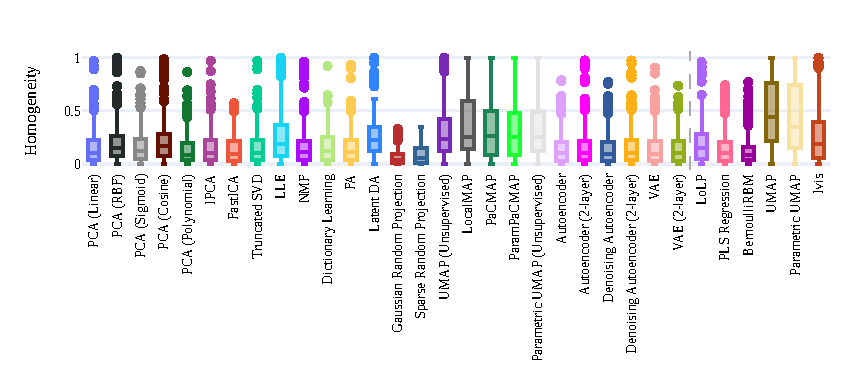
\includegraphics[width=\textwidth]{figures/04/ml/agg_5_homogeneity.pdf}
        \caption{\footnotesize{$k = 5$; homogeneity}}
    \end{subfigure}
    \begin{subfigure}{0.24\textwidth}
        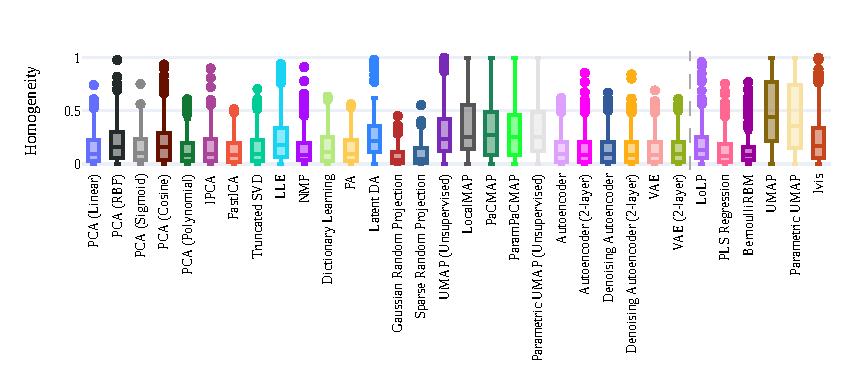
\includegraphics[width=\textwidth]{figures/04/ml/agg_10_homogeneity.pdf}
        \caption{\footnotesize{$k = 10$; homogeneity}}
    \end{subfigure}
    \begin{subfigure}{0.24\textwidth}
        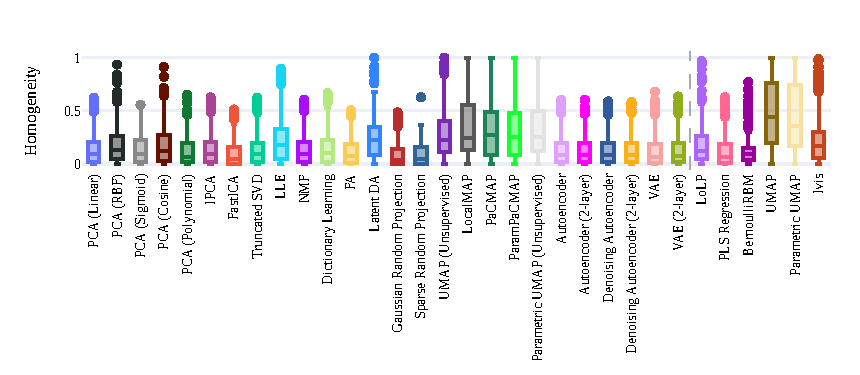
\includegraphics[width=\textwidth]{figures/04/ml/agg_20_homogeneity.pdf}
        \caption{\footnotesize{$k = 20$; homogeneity}}
    \end{subfigure}
    \begin{subfigure}{0.24\textwidth}
        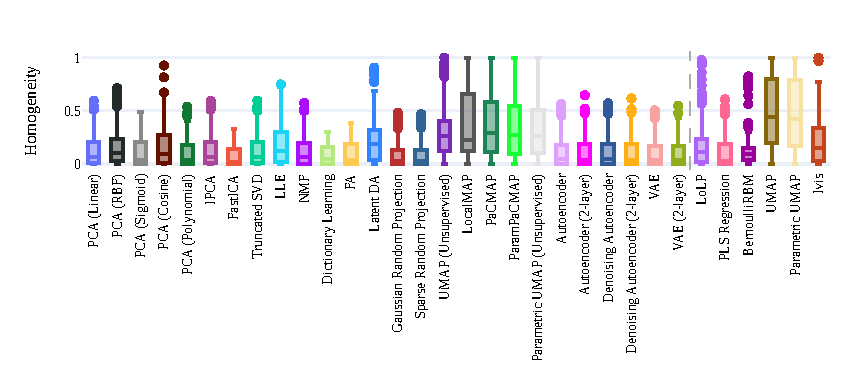
\includegraphics[width=\textwidth]{figures/04/ml/agg_40_homogeneity.pdf}
        \caption{\footnotesize{$k = 40$; homogeneity}}
    \end{subfigure}
    \begin{subfigure}{0.24\textwidth}
        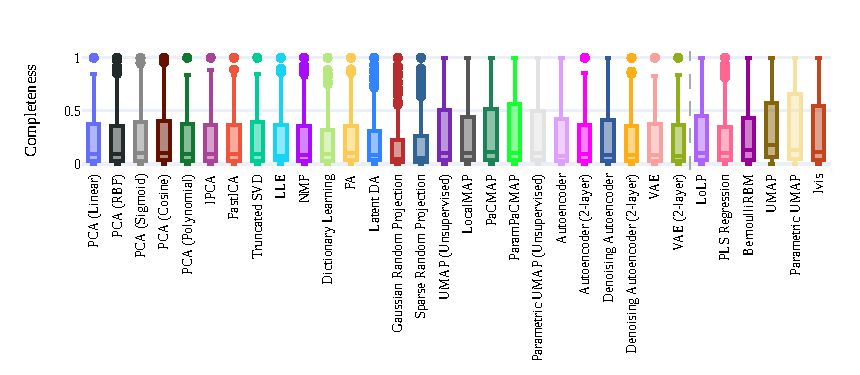
\includegraphics[width=\textwidth]{figures/04/ml/agg_5_completeness.pdf}
        \caption{\footnotesize{$k = 5$; completeness}}
    \end{subfigure}
    \begin{subfigure}{0.24\textwidth}
        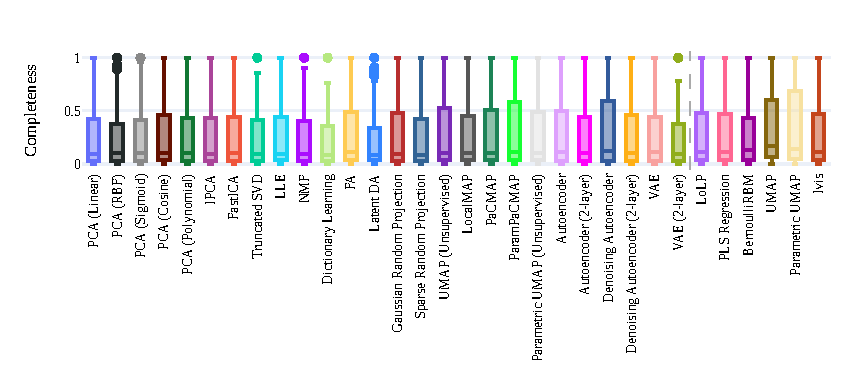
\includegraphics[width=\textwidth]{figures/04/ml/agg_10_completeness.pdf}
        \caption{\footnotesize{$k = 10$; completeness}}
    \end{subfigure}
    \begin{subfigure}{0.24\textwidth}
        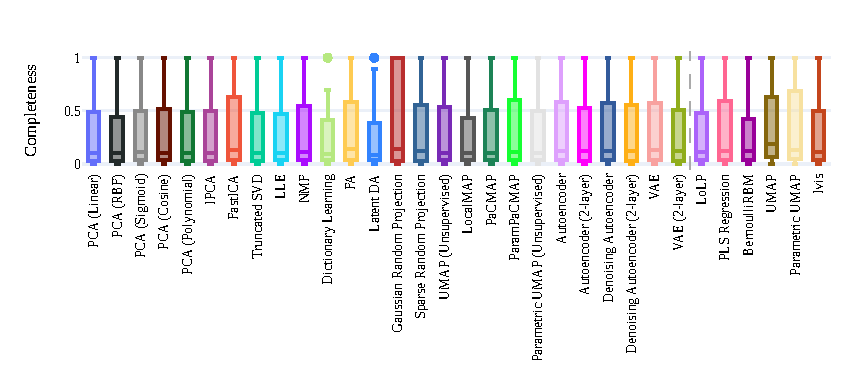
\includegraphics[width=\textwidth]{figures/04/ml/agg_20_completeness.pdf}
        \caption{\footnotesize{$k = 20$; completeness}}
    \end{subfigure}
    \begin{subfigure}{0.24\textwidth}
        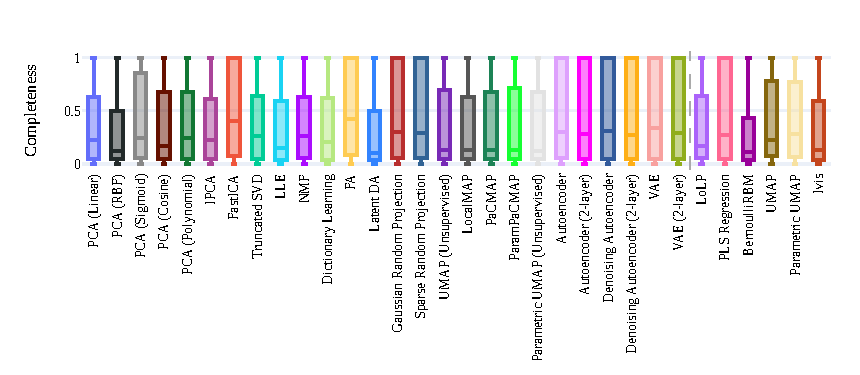
\includegraphics[width=\textwidth]{figures/04/ml/agg_40_completeness.pdf}
        \caption{\footnotesize{$k = 40$; completeness}}
    \end{subfigure}




















\caption[Clustering homogeneity and completeness on ML task 1]{

Performance of different dimensionality reduction methods aggregated across all OpenML~CC-18 datasets, for different target dimensionalities $k$, in terms of (a-d) cluster homogeneity and (e-h) cluster completeness on \textbf{machine learning task 1: clustering ability}; higher is better. Homogeneity measures whether each cluster contains samples from the same true class; we observe very small homogeneity differences between dimensionality reduction methods for different target dimensionalities. Completeness quantifies whether all samples belonging to the same true class are in the same cluster; we observe a slight improvement in performance measured by completeness as the target dimensionality increases.

}
\label{fig:ch04:cluster_all_agg}
\end{figure}

We now investigate the effect of input dimensionality by grouping the datasets into three categories based on their number of features: low- (up to 60 features), medium- (60–200 features), and high-dimensional datasets (more than 200 features). The results are presented in \cref{fig:ch04:cluster_homogeneity_dataset_sizes}.
We observe that LLE performs increasingly well on both metrics as the input dimensionality grows, reaching its best performance on medium-dimensional datasets.


This is possibly due to interference between the fact that some dimensions are irrelevant in the large-sized datasets and the estimation of a local neighbourhood.




With respect to cluster completeness, sparse random projection performs best on medium-dimensional data, whereas Gaussian random projection becomes the strongest method for large input dimensionalities, likely due to its ability to better preserve pairwise distances in high dimensions, consistent with the Johnson–Lindenstrauss effect.
Furthermore, dense Gaussian random projections handle large feature spaces better than sparse ones, avoiding information loss in very high dimensions.

\begin{figure}
\centering
    \begin{subfigure}{0.32\textwidth}
        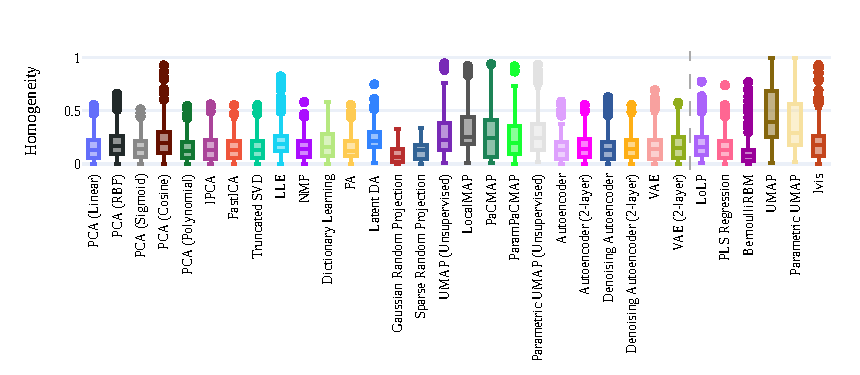
\includegraphics[width=\textwidth]{figures/04/ml/agg_small_5_homogeneity.pdf}
        \caption{Small $D$; homogeneity}
    \end{subfigure}
    \begin{subfigure}{0.32\textwidth}
        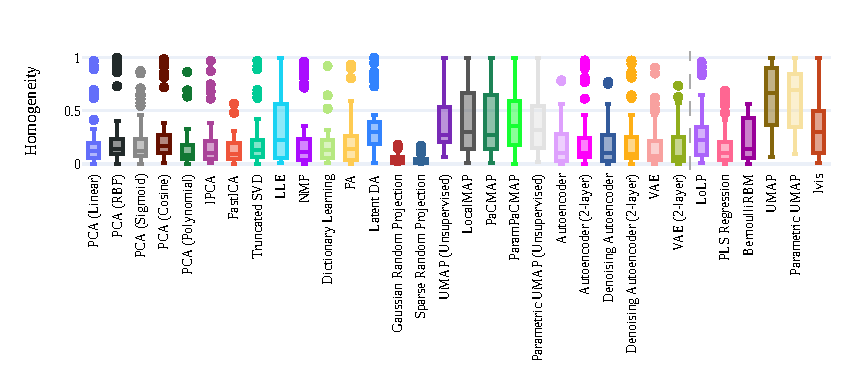
\includegraphics[width=\textwidth]{figures/04/ml/agg_medium_5_homogeneity.pdf}
        \caption{Medium $D$; homogeneity}
    \end{subfigure}
    \begin{subfigure}{0.32\textwidth}
        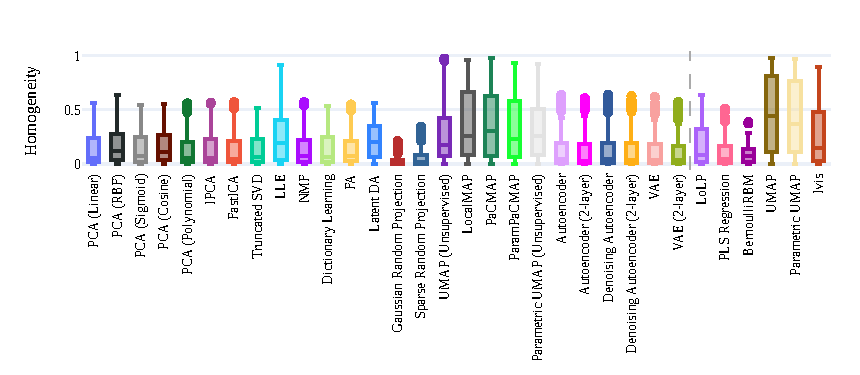
\includegraphics[width=\textwidth]{figures/04/ml/agg_large_5_homogeneity.pdf}
        \caption{Large $D$; homogeneity}
    \end{subfigure}
    \begin{subfigure}{0.32\textwidth}
        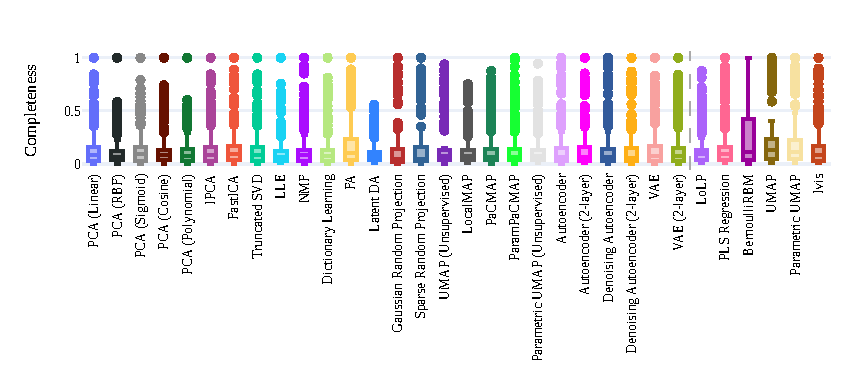
\includegraphics[width=\textwidth]{figures/04/ml/agg_small_5_completeness.pdf}
        \caption{Small $D$; completeness}
    \end{subfigure}
    \begin{subfigure}{0.32\textwidth}
        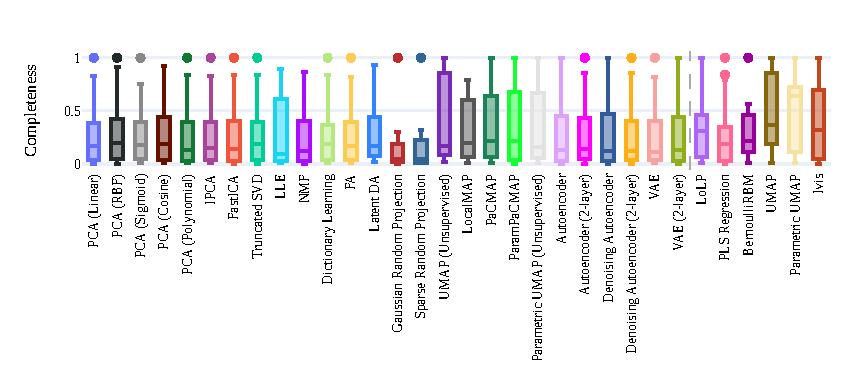
\includegraphics[width=\textwidth]{figures/04/ml/agg_medium_5_completeness.pdf}
        \caption{Medium $D$; completeness}
    \end{subfigure}
    \begin{subfigure}{0.32\textwidth}
        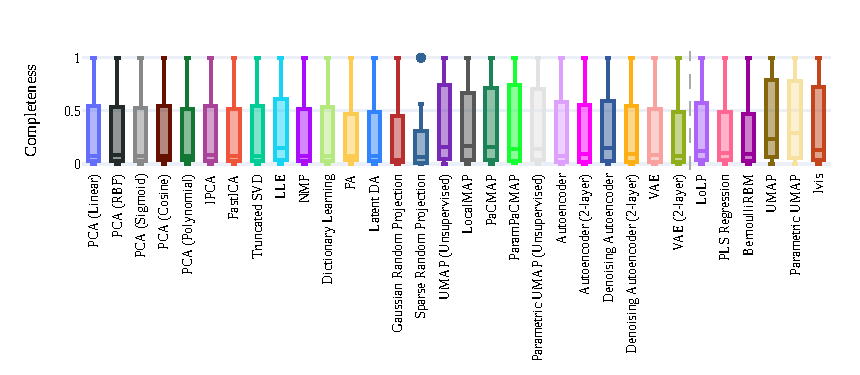
\includegraphics[width=\textwidth]{figures/04/ml/agg_large_5_completeness.pdf}
        \caption{Large $D$; completeness}
    \end{subfigure}
    \begin{subfigure}{0.32\textwidth}










    \end{subfigure}




\caption[Clustering on ML task 1 by dataset category]{

Performance of different dimensionality reduction methods on low-, medium- and high-dimensional OpenML~CC-18 datasets, all reduced to target dimensionality $k = 5$, in terms of (a-c) cluster homogeneity and (d-f) cluster completeness on \textbf{machine learning task 1: clustering ability}; higher is better. We observe a slightly larger improvement in completeness than in homogeneity as the dataset dimensionality increases.


}
\label{fig:ch04:cluster_homogeneity_dataset_sizes}
\end{figure}



\subsubsection*{Machine learning task 2: Tabular classification accuracy}



For the supervised machine learning task (\emph{i.e.,} prediction), 

we begin by analysing the results aggregated across all datasets and different machine learning models (random forest, gradient boosting, \gls{mlp}) for varying target dimensionalities $k$, as shown in \cref{fig:ch04:ml_pred_all}.
Across all models and methods, we observe that accuracy increases with the target dimensionality. 


In other words,


performance is lowest at $k=5$ and highest at $k=40$. 
This observation indicates that higher-dimensional projections retain more task-relevant information, allowing downstream models to make more accurate predictions.

Interestingly, while Gaussian and sparse random projection performed relatively well in the clustering task (particularly for cluster completeness), they rank among the worst-performing methods in the prediction task, only outperforming Bernoulli RBM. This suggests that although random projections preserve geometric structure, they do not necessarily retain the discriminative information required for predictive modelling.
Overall, while most methods achieve comparable accuracy, LoLP consistently performs best. This outcome is expected, as LoLP is explicitly designed to enhance predictive performance in machine learning settings, confirming its suitability for supervised downstream tasks.


\begin{figure}
\centering
    \begin{subfigure}{0.24\textwidth}
        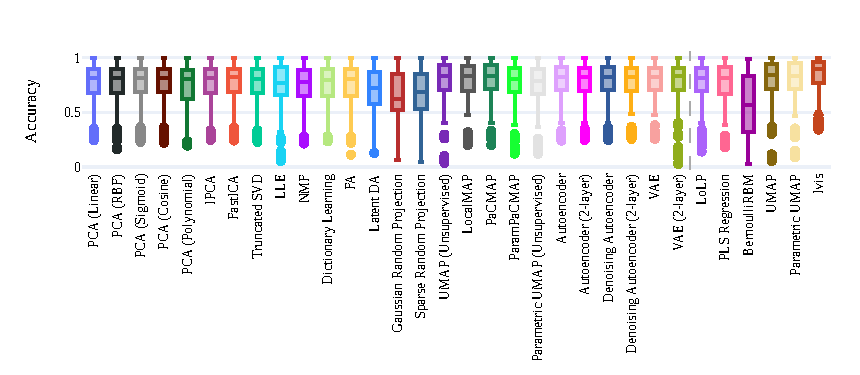
\includegraphics[width=\textwidth]{figures/04/ml/agg_5_rf_acc.pdf}
        \caption{\footnotesize Random Forest; $k = 5$}
    \end{subfigure}
    \begin{subfigure}{0.24\textwidth}
        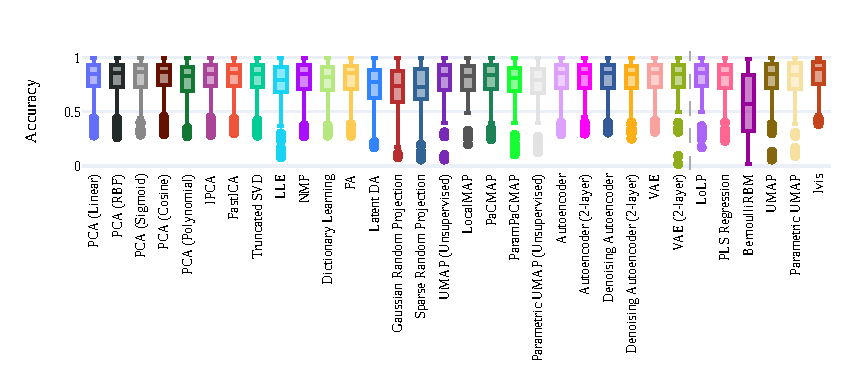
\includegraphics[width=\textwidth]{figures/04/ml/agg_10_rf_acc.pdf}
        \caption{\footnotesize Random Forest; $k = 10$}
    \end{subfigure}
    \begin{subfigure}{0.24\textwidth}
        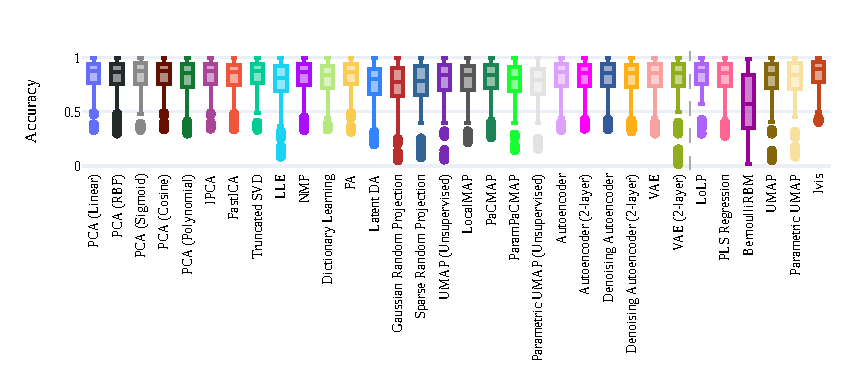
\includegraphics[width=\textwidth]{figures/04/ml/agg_20_rf_acc.pdf}
        \caption{\footnotesize Random Forest; $k = 20$}
    \end{subfigure}
    \begin{subfigure}{0.24\textwidth}
        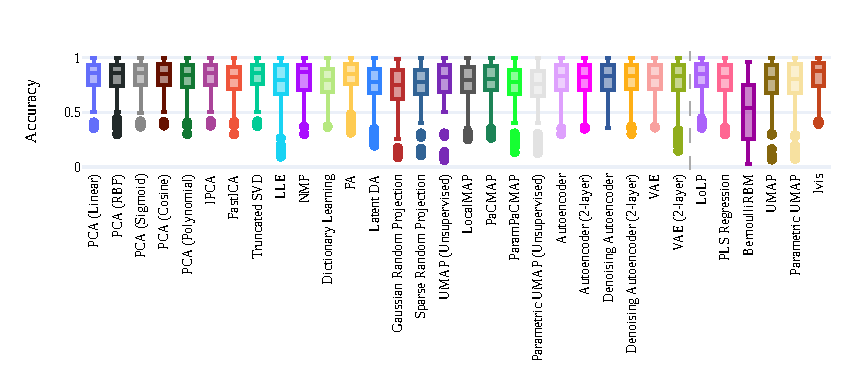
\includegraphics[width=\textwidth]{figures/04/ml/agg_40_rf_acc.pdf}
        \caption{\footnotesize Random Forest; $k = 40$}
    \end{subfigure}
    \begin{subfigure}{0.24\textwidth}
        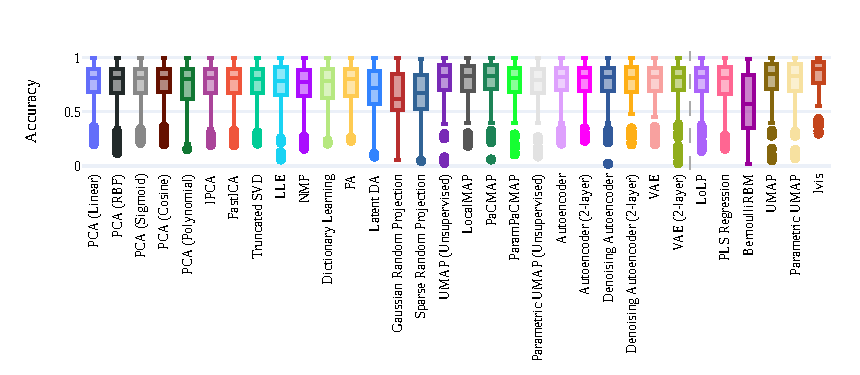
\includegraphics[width=\textwidth]{figures/04/ml/agg_5_gb_acc.pdf}
        \caption{\footnotesize Gradient Boosting; $k = 5$}
    \end{subfigure}
    \begin{subfigure}{0.24\textwidth}
        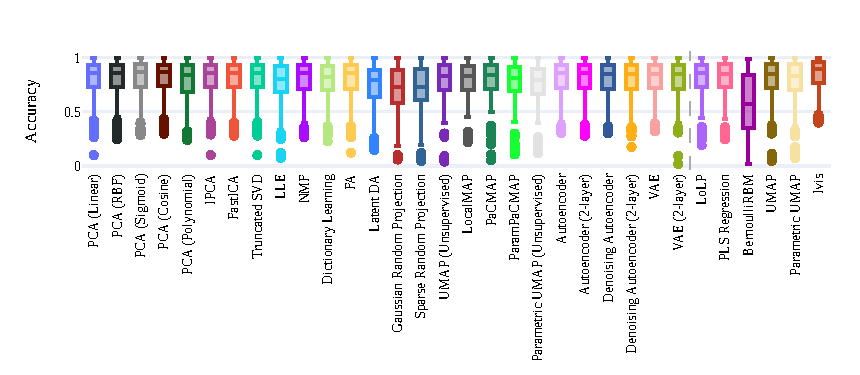
\includegraphics[width=\textwidth]{figures/04/ml/agg_10_gb_acc.pdf}
        \caption{\footnotesize Gradient Boosting; $k = 10$}
    \end{subfigure}
    \begin{subfigure}{0.24\textwidth}
        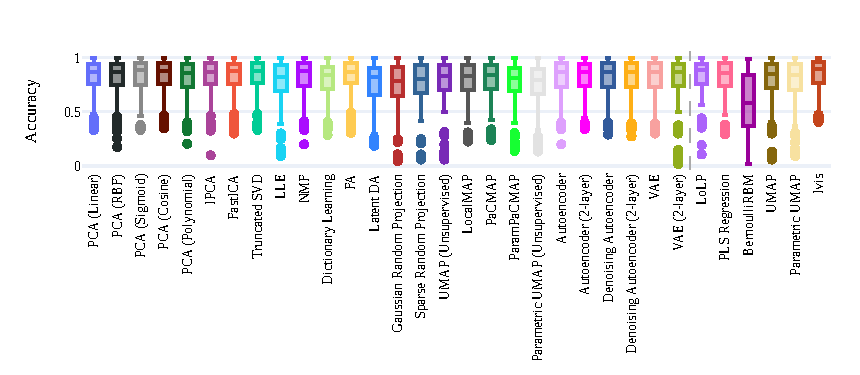
\includegraphics[width=\textwidth]{figures/04/ml/agg_20_gb_acc.pdf}
        \caption{\footnotesize Gradient Boosting; $k = 20$}
    \end{subfigure}
    \begin{subfigure}{0.24\textwidth}
        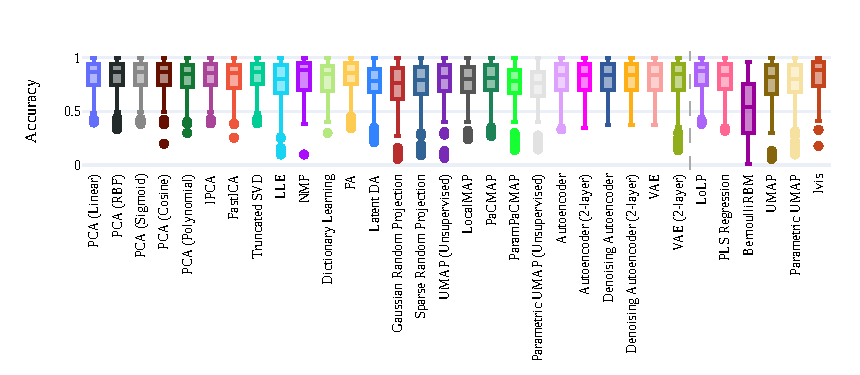
\includegraphics[width=\textwidth]{figures/04/ml/agg_40_gb_acc.pdf}
        \caption{\footnotesize Gradient Boosting; $k = 40$}
    \end{subfigure}
    \begin{subfigure}{0.24\textwidth}
        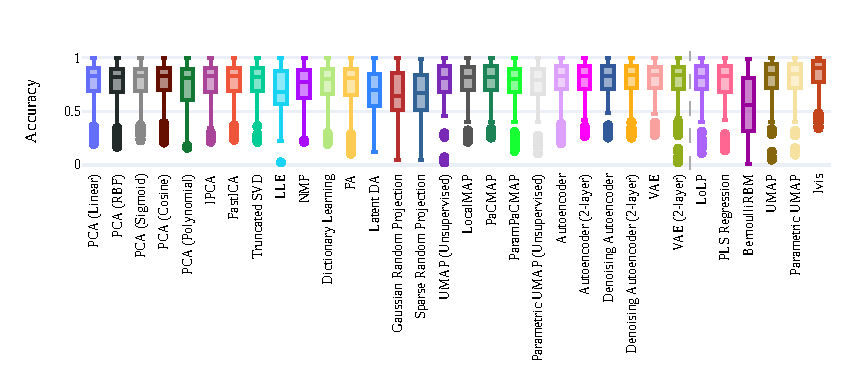
\includegraphics[width=\textwidth]{figures/04/ml/agg_5_mlp_acc.pdf}
        \caption{\footnotesize \gls{mlp}; $k = 5$}
    \end{subfigure}
    \begin{subfigure}{0.24\textwidth}
        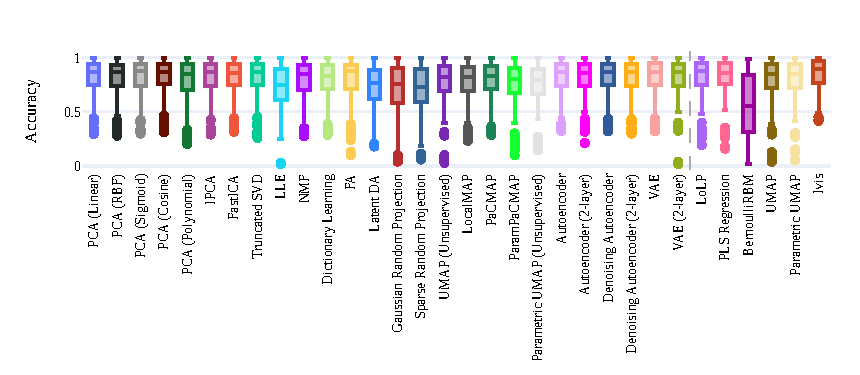
\includegraphics[width=\textwidth]{figures/04/ml/agg_10_mlp_acc.pdf}
        \caption{\footnotesize \gls{mlp}; $k = 10$}
    \end{subfigure}
    \begin{subfigure}{0.24\textwidth}
        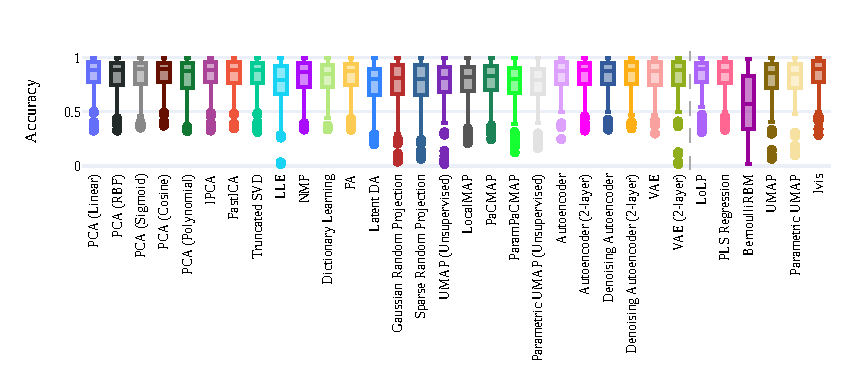
\includegraphics[width=\textwidth]{figures/04/ml/agg_20_mlp_acc.pdf}
        \caption{\footnotesize \gls{mlp}; $k = 20$}
    \end{subfigure}
    \begin{subfigure}{0.24\textwidth}
        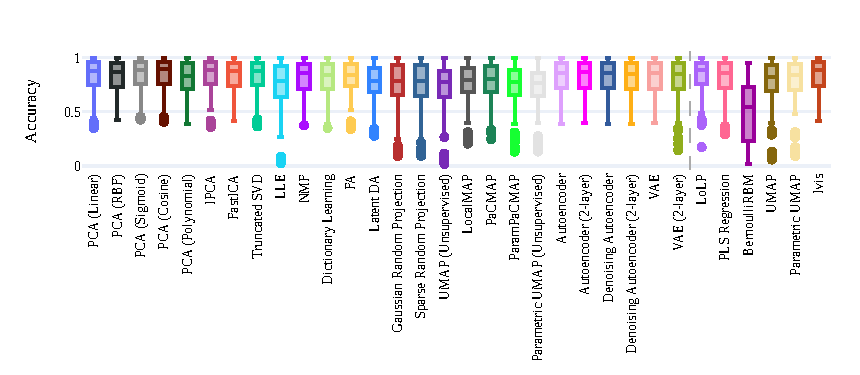
\includegraphics[width=\textwidth]{figures/04/ml/agg_40_mlp_acc.pdf}
        \caption{\footnotesize \gls{mlp}; $k = 40$}
    \end{subfigure}




\caption[Classification accuracy on ML task 2]{

Performance of different dimensionality reduction methods aggregated across all OpenML~CC-18 datasets, for different target dimensionalities $k$ and for different machine learning models used for classification (random forest, gradient boosting, \gls{mlp}), in terms of accuracy on \textbf{machine learning task 2: tabular classification accuracy}; higher is better. Bernoulli RBM performs consistently bad across all settings, followed by Gaussian and sparse random projections, while LoLP exhibits a consistent slight performance edge over other methods.

}
\label{fig:ch04:ml_pred_all}
\end{figure}

We conclude our analysis of the machine learning tasks by examining the results of the prediction task across different dataset sizes, following the same procedure as for the clustering task. We fix the target dimensionality to $k=5$.

We first observe that Bernoulli RBM, Gaussian and sparse random projections show strongly degraded performance as the number of features increases. Even on the low-dimensional datasets, these methods already underperform compared to other approaches, suggesting that they increasingly fail to preserve essential information needed for predictive modelling as dataset dimensionality increases.
In contrast, PCA (Linear) and PCA (Polynomial) perform better than other PCA variants on low-dimensional datasets. This behaviour likely reflects that linear and low-order polynomial relationships are sufficient to capture the main predictive variance in smaller feature spaces, while more complex kernels (such as RBF or Cosine) become beneficial only in higher-dimensional spaces.

\begin{figure}
\centering
    \begin{subfigure}{0.32\textwidth}
        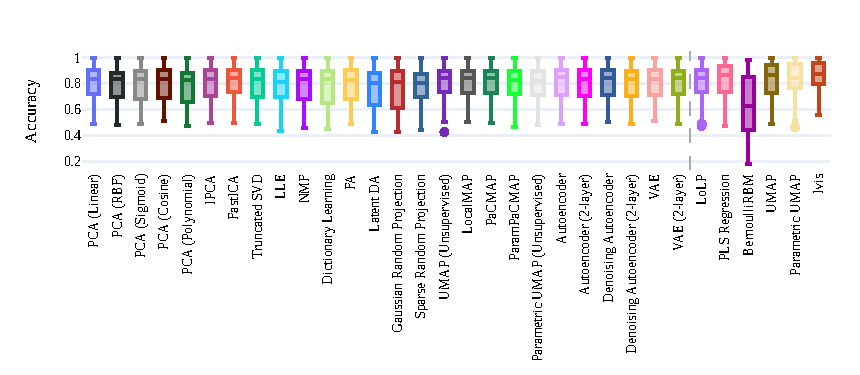
\includegraphics[width=\textwidth]{figures/04/ml/agg_small_5_rf_acc.pdf}
        \caption{Small $D$; Random Forest}
    \end{subfigure}
    \begin{subfigure}{0.32\textwidth}
        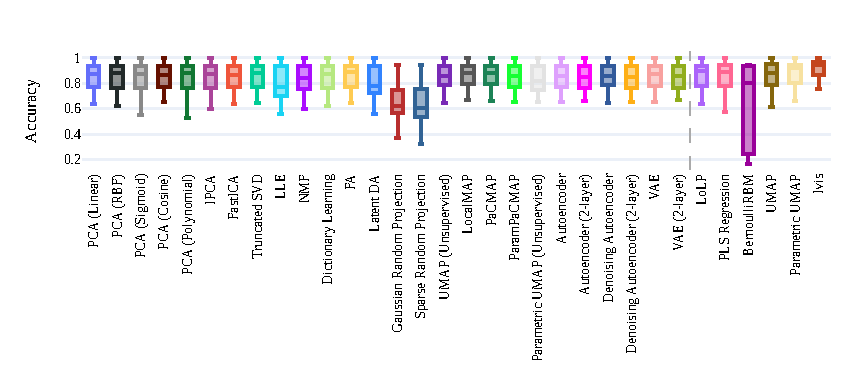
\includegraphics[width=\textwidth]{figures/04/ml/agg_medium_5_rf_acc.pdf}
        \caption{Medium $D$; Random Forest}
    \end{subfigure}
    \begin{subfigure}{0.32\textwidth}
        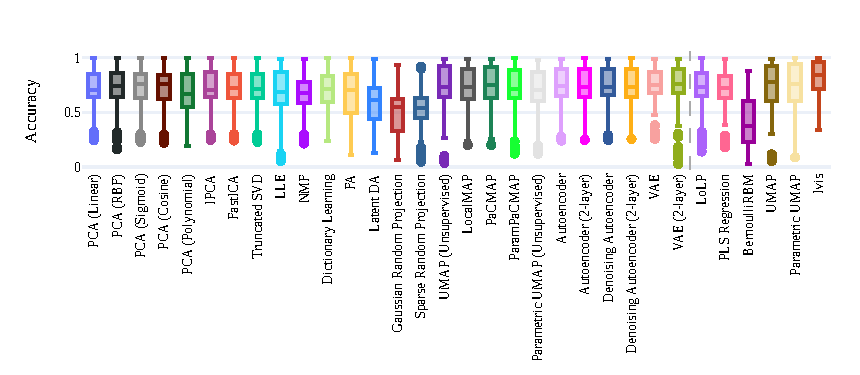
\includegraphics[width=\textwidth]{figures/04/ml/agg_large_5_rf_acc.pdf}
        \caption{Large $D$; Random Forest}
    \end{subfigure}
    \begin{subfigure}{0.32\textwidth}
        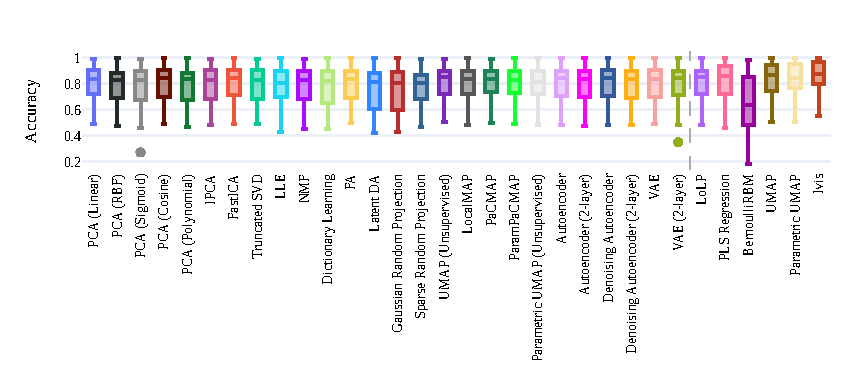
\includegraphics[width=\textwidth]{figures/04/ml/agg_small_5_gb_acc.pdf}
        \caption{Small $D$; Gradient Boosting}
    \end{subfigure}
    \begin{subfigure}{0.32\textwidth}
        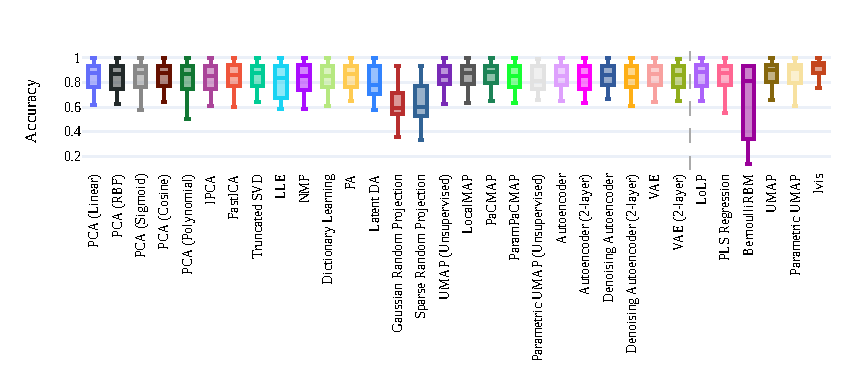
\includegraphics[width=\textwidth]{figures/04/ml/agg_medium_5_gb_acc.pdf}
        \caption{Medium $D$; Gradient Boosting}
    \end{subfigure}
    \begin{subfigure}{0.32\textwidth}
        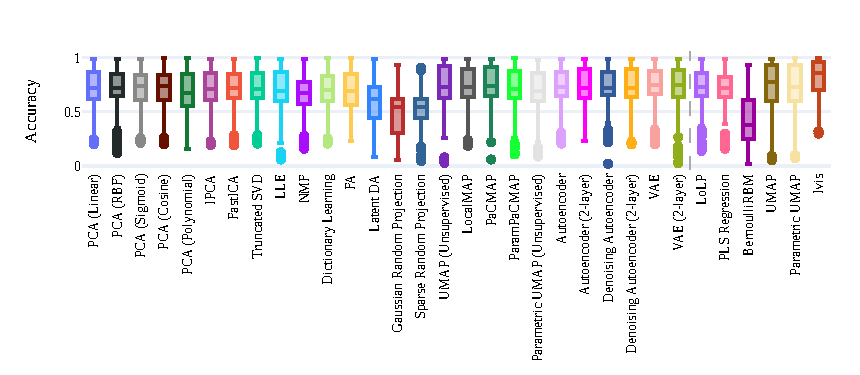
\includegraphics[width=\textwidth]{figures/04/ml/agg_large_5_gb_acc.pdf}
        \caption{Large $D$; Gradient Boosting}
    \end{subfigure}
    \begin{subfigure}{0.32\textwidth}
        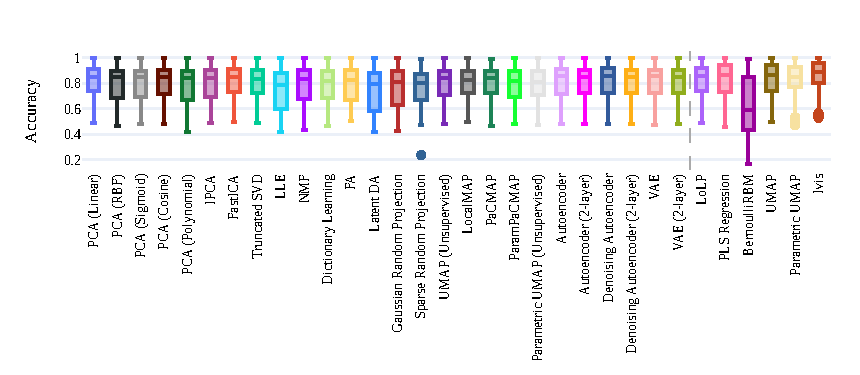
\includegraphics[width=\textwidth]{figures/04/ml/agg_small_5_mlp_acc.pdf}
        \caption{Small $D$; \gls{mlp}}
    \end{subfigure}
    \begin{subfigure}{0.32\textwidth}
        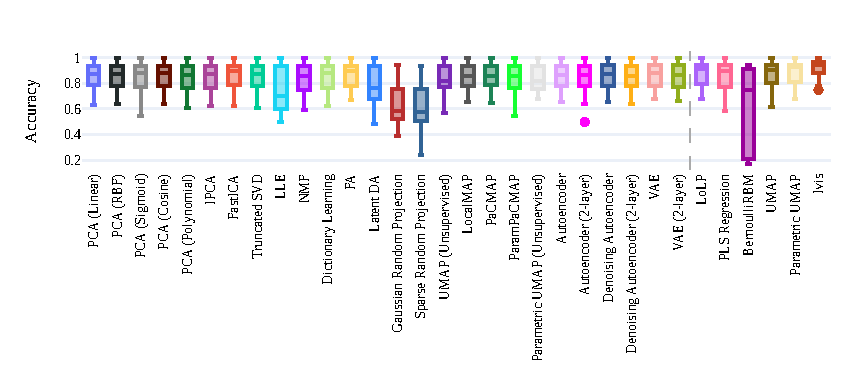
\includegraphics[width=\textwidth]{figures/04/ml/agg_medium_5_mlp_acc.pdf}
        \caption{Medium $D$; \gls{mlp}}
    \end{subfigure}
    \begin{subfigure}{0.32\textwidth}
        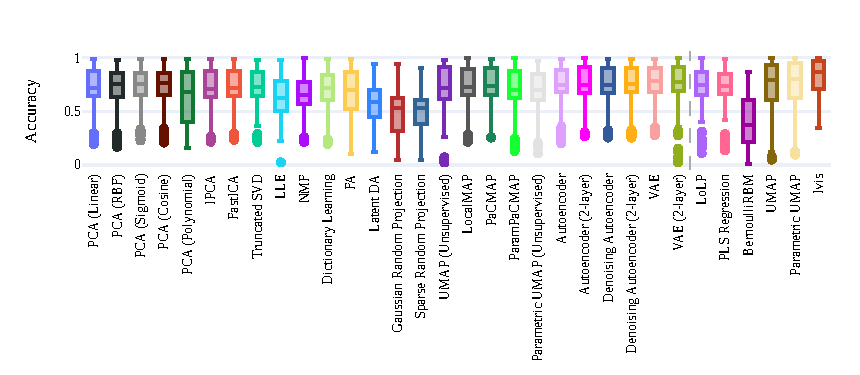
\includegraphics[width=\textwidth]{figures/04/ml/agg_large_5_mlp_acc.pdf}
        \caption{Large $D$; \gls{mlp}}
    \end{subfigure}





\caption[Classification accuracy on ML task 2 by dataset category]{

Performance of different dimensionality reduction methods on low-, medium- and high-dimensional OpenML~CC-18 datasets, all reduced to target dimensionality $k = 5$, in terms of accuracy on \textbf{machine learning task 2: tabular classification accuracy}, where classification is done using different machine learning models (random forest, gradient boosting, \gls{mlp}); higher is better. The performance of Bernoulli RBM and Gaussian and sparse random projection degrades even further as the dataset dimensionality increases, regardless of the machine learning model used for classification. The differences induced by the choice of the machine learning model are generally negligible for low-, medium- and high-dimensional datasets alike.

}
\label{fig:ch04:ml_pred_sizes}
\end{figure}


\subsection{Black-box optimisation tasks}
\label{sec:ch04:res-bbo}

\subsubsection*{Black-box optimisation task 1: Target function approximation}






\begin{figure}
    \centering
    \begin{subfigure}[t]{0.24\textwidth}
        \centering
        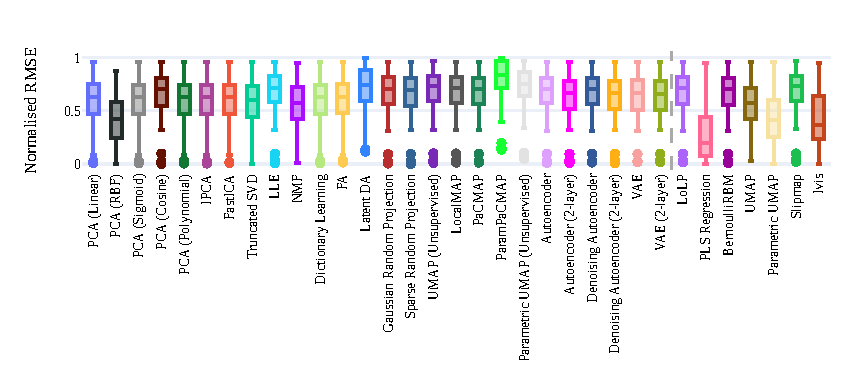
\includegraphics[width=\textwidth]{figures/04/epm/agg_sample_red_inpt_100_120_5.pdf}
        \caption{$k=5$}
    \end{subfigure}
    \begin{subfigure}[t]{0.24\textwidth}
        \centering
        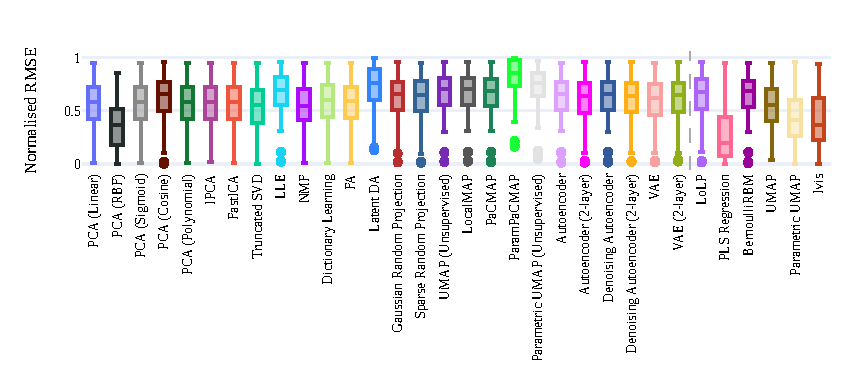
\includegraphics[width=\textwidth]{figures/04/epm/agg_sample_red_inpt_100_120_10.pdf}
        \caption{$k=10$}
    \end{subfigure}
    \begin{subfigure}[t]{0.24\textwidth}
        \centering
        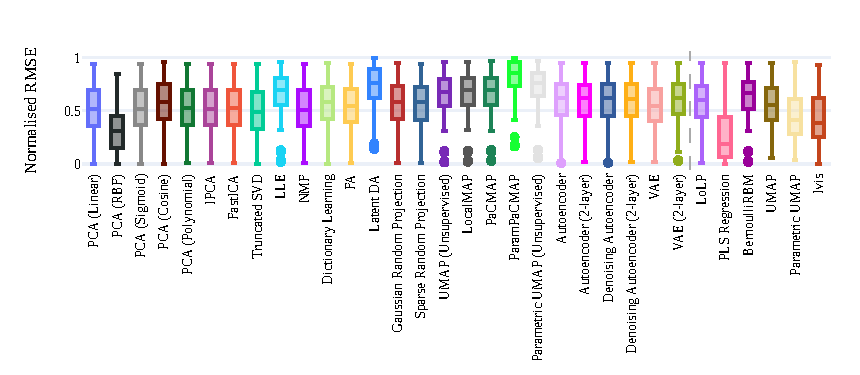
\includegraphics[width=\textwidth]{figures/04/epm/agg_sample_red_inpt_100_120_20.pdf}
        \caption{$k=20$}
    \end{subfigure}
    \begin{subfigure}[t]{0.24\textwidth}
        \centering
        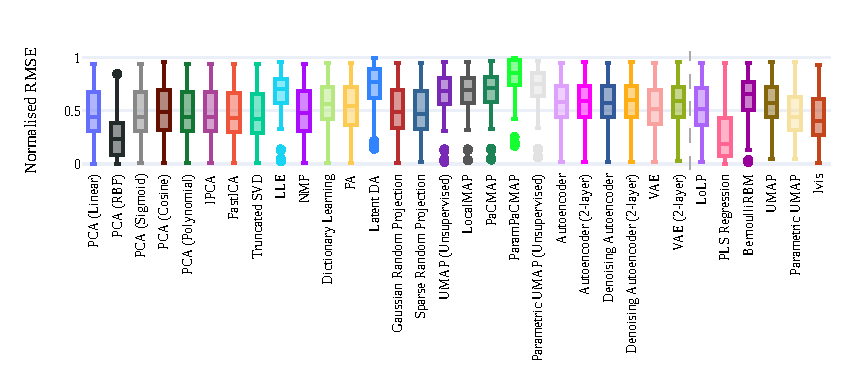
\includegraphics[width=\textwidth]{figures/04/epm/agg_sample_red_inpt_100_120_40.pdf}
        \caption{$k=40$}
    \end{subfigure}
    \caption[Target function approximation on BBO task 1]{

    Performance of different dimensionality reduction methods aggregated across synthetic benchmark problems for different target dimensionalities $k$, with input dimensionality $D = 120$ and initial sample size $N = 100$, in terms of min-max normalised mean \gls{rmse} on \textbf{black-box optimisation task 1: target function approximation}; lower is better. 
    PLS regression consistently performs best across different target dimensionalities, and is closely followed by PCA (RBF) for the highest target dimensionality.



    }
    \label{fig:ch04:res-bbo-task1_red_dim_inpt_dim}
\end{figure}


We focus on a selection of representative aggregated results to simplify analysis.
We start by looking into the results on synthetic benchmarks for black-box optimisation task 1.


First, we examine the effect of varying the target dimensionality $k$ in \cref{fig:ch04:res-bbo-task1_red_dim_inpt_dim}, keeping the input dimensionality fixed at $D = 120$ and the initial sample size at $N = 100$.
Across all target dimensionalities, and particularly in the low-dimensional setting, PLS regression consistently performs best. 
This aligns with expectations, as PLS components are explicitly optimised to maximise the predictive power of the target variables, which is especially suitable when dimensionality reduction is used as a preprocessing step for regression. 

As the target dimensionality increases, PCA (RBF) gradually catches up and eventually performs on par with PLS regression. More generally, all PCA variants improve their relative performance with higher target dimensionalities, likely because higher-dimensional projections preserve more variance and structure from the original data, even without explicit supervision.



\begin{figure}
\begin{subfigure}[t]{0.32\textwidth}
        \centering
        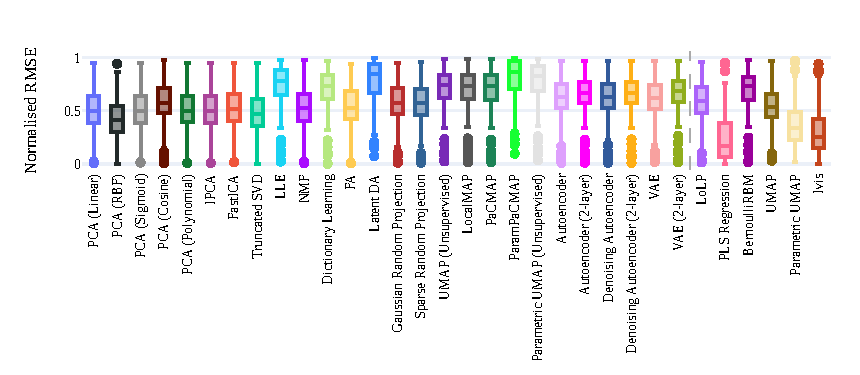
\includegraphics[width=\textwidth]{figures/04/epm/agg_sample_red_inpt_100_40_20.pdf}
        \caption{$D=40$}
    \end{subfigure}
    \begin{subfigure}[t]{0.32\textwidth}
        \centering
        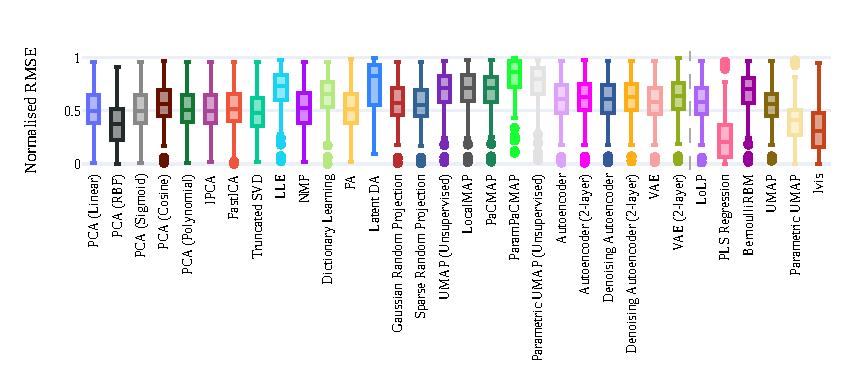
\includegraphics[width=\textwidth]{figures/04/epm/agg_sample_red_inpt_100_60_20.pdf}
        \caption{$D=60$}
    \end{subfigure}
    \begin{subfigure}[t]{0.32\textwidth}
        \centering
        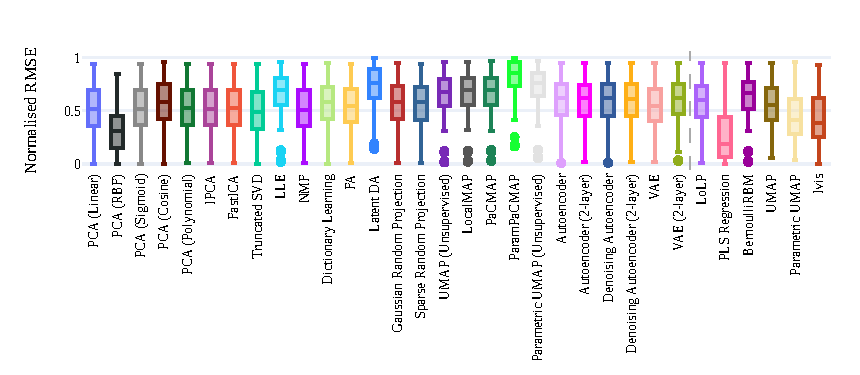
\includegraphics[width=\textwidth]{figures/04/epm/agg_sample_red_inpt_100_120_20.pdf}
        \caption{$D=120$}
    \end{subfigure}
    \begin{subfigure}[t]{0.32\textwidth}
        \centering
        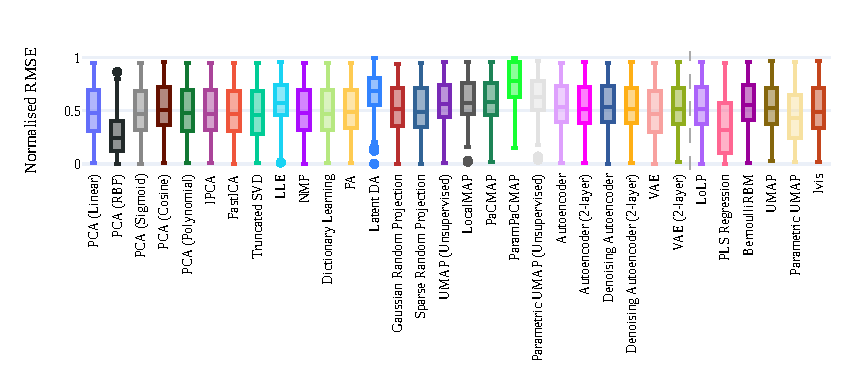
\includegraphics[width=\textwidth]{figures/04/epm/agg_sample_red_inpt_100_240_20.pdf}
        \caption{$D=240$}
    \end{subfigure}
    \begin{subfigure}[t]{0.32\textwidth}
        \centering
        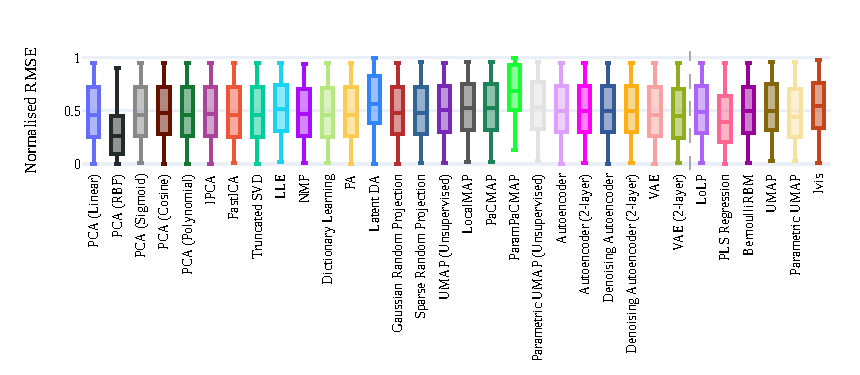
\includegraphics[width=\textwidth]{figures/04/epm/agg_sample_red_inpt_100_500_20.pdf}
        \caption{$D=500$}
    \end{subfigure}
    \begin{subfigure}[t]{0.32\textwidth}
        \centering
        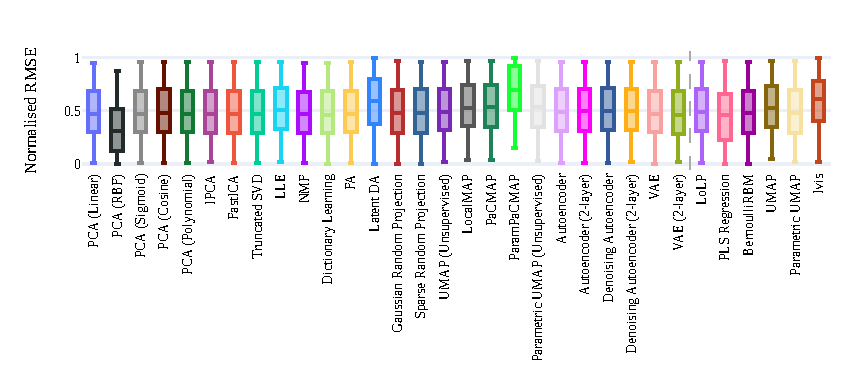
\includegraphics[width=\textwidth]{figures/04/epm/agg_sample_red_inpt_100_1000_20.pdf}
        \caption{$D=1000$}
    \end{subfigure}
    \hspace{0.2cm}
    \begin{subfigure}[t]{0.8\textwidth}
        \centering
        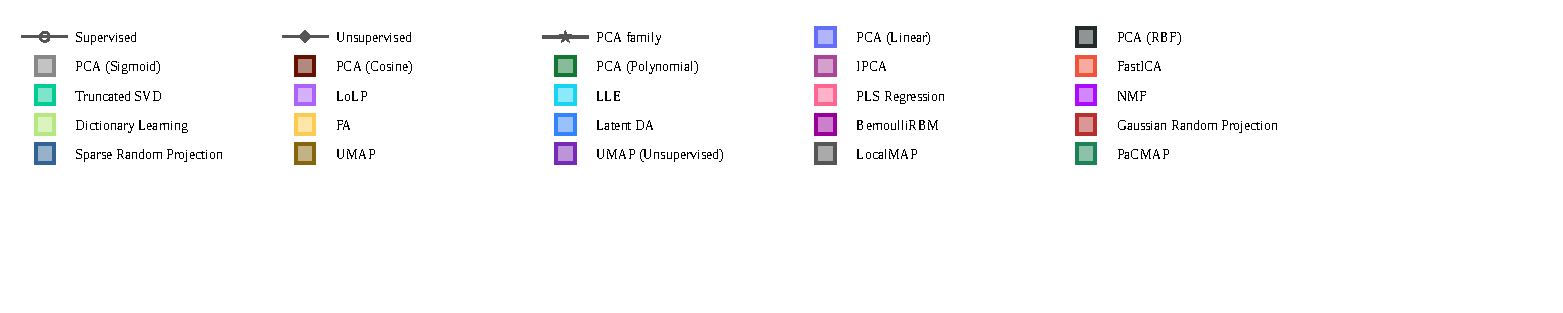
\includegraphics[width=1.0\textwidth,trim={1.5cm 4cm 3.7cm 0.0cm},clip]{figures/04/legend.pdf}
    \end{subfigure}
    \caption[Target function approximation on BBO task 1 for real-world benchmarks]{

    Performance of different dimensionality reduction methods aggregated across synthetic benchmark problems for different input dimensionalities $D$, with target dimensionality $k = 20$ and initial sample size $N = 100$, in terms of min-max normalised mean \gls{rmse} on \textbf{black-box optimisation task 1: target function approximation}; lower is better. 
    The variance increases with input dimensionality; PLS regression is a dominant method for lower-dimensional inputs (a-c), but is outperformed by PCA (RBF) for higher-dimensional inputs (d-f).


    }
    \label{fig:ch04:res-bbo-task1_inpt_dim}
\end{figure}



Second, we look into the effect of varying the input dimensionality $D$, keeping the target dimensionality fixed at $k = 20$ and the initial sample size at $N = 100$. This is illustrated in~\cref{fig:ch04:res-bbo-task1_inpt_dim}.


As expected, the variance of all methods decreases with lower input dimensionality, reflecting the reduced complexity of the search space. In this setting (up to ~120 input dimensions), PLS regression consistently outperforms other methods, leveraging its ability to extract components that are directly predictive of the targets. Conversely, for higher input dimensionalities, PCA (RBF) becomes the dominant method, likely because it captures more of the underlying variance and non-linear structure that PLS regression cannot exploit efficiently in very high-dimensional spaces. Together with previous findings, this suggests that PLS regression is best when both input and output dimensions are small, while PCA (RBF) is more suitable for high-dimensional settings.



\begin{figure}
    \centering
    \begin{subfigure}[t]{0.24\textwidth}
        \centering
        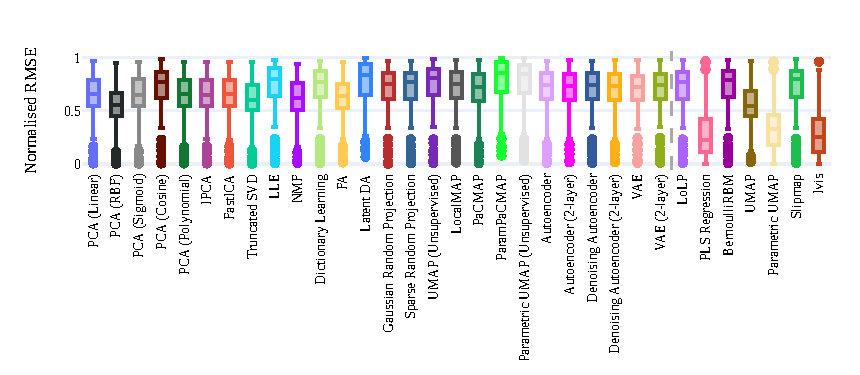
\includegraphics[width=\textwidth]{figures/04/epm/agg_sample_red_inpt_100_40_5}
        \caption{\footnotesize$D = 40, k = 5, N = 100$}
    \end{subfigure}
    \begin{subfigure}[t]{0.24\textwidth}
        \centering
        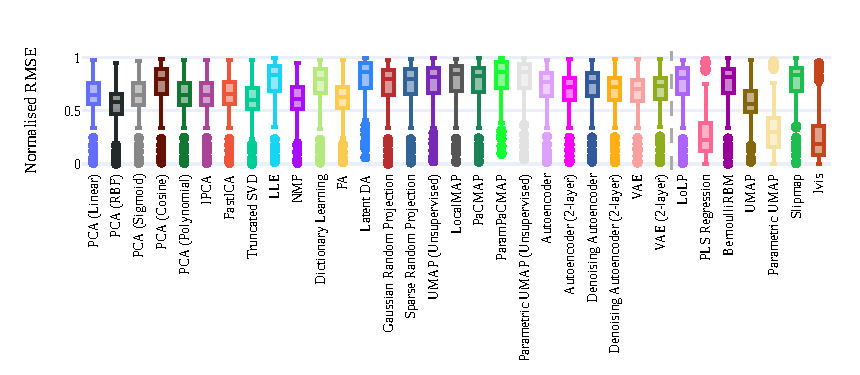
\includegraphics[width=\textwidth]{figures/04/epm/agg_sample_red_inpt_200_40_5.pdf}
        \caption{\footnotesize$D = 40, k = 5, N = 200$}
    \end{subfigure}
    \begin{subfigure}[t]{0.24\textwidth}
        \centering
        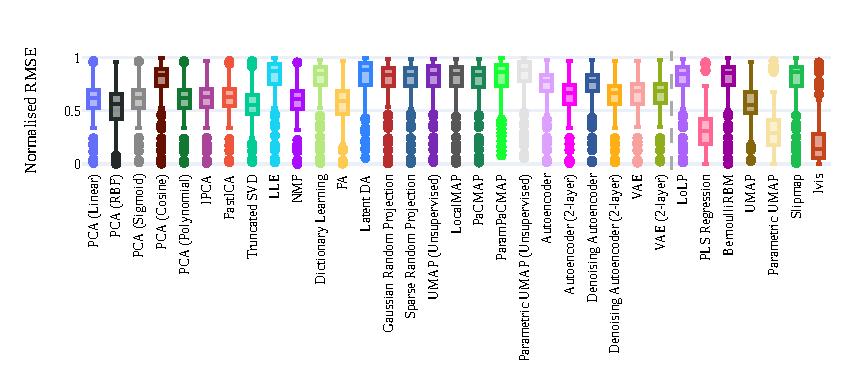
\includegraphics[width=\textwidth]{figures/04/epm/agg_sample_red_inpt_500_40_5.pdf}
        \caption{\footnotesize$D = 40, k = 5, N = 500$}
    \end{subfigure}
    \begin{subfigure}[t]{0.24\textwidth}
        \centering
        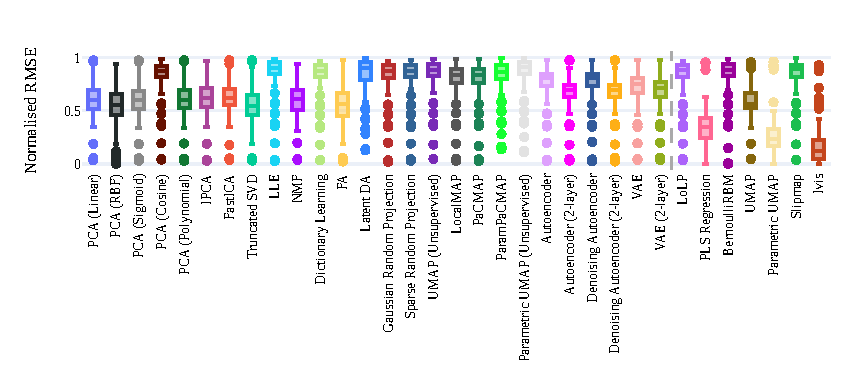
\includegraphics[width=\textwidth]{figures/04/epm/agg_sample_red_inpt_1000_40_5.pdf}
        \caption{\footnotesize$D = 40, k = 5, N = 1000$}
    \end{subfigure}
    \begin{subfigure}[t]{0.24\textwidth}
        \centering
        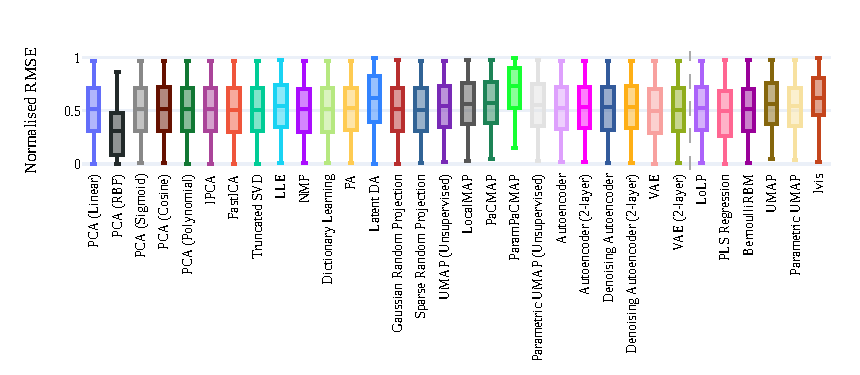
\includegraphics[width=\textwidth]{figures/04/epm/agg_sample_red_inpt_100_1000_40.pdf}
        \caption{\footnotesize$D = 1000, k = 40, N = 100$}
    \end{subfigure}
    \begin{subfigure}[t]{0.24\textwidth}
        \centering
        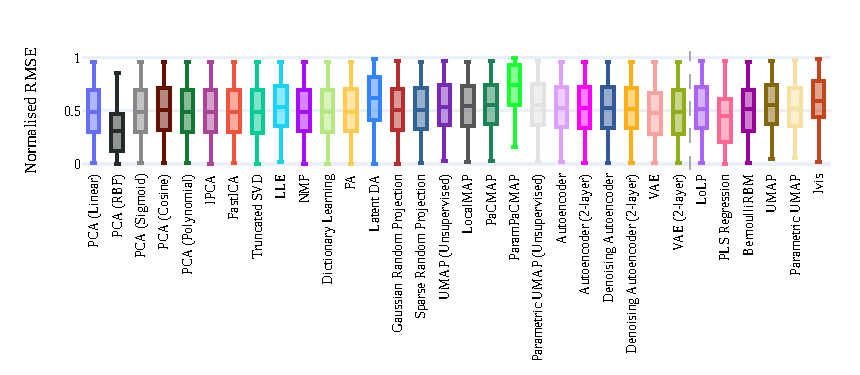
\includegraphics[width=\textwidth]{figures/04/epm/agg_sample_red_inpt_200_1000_40.pdf}
        \caption{\footnotesize$D = 1000, k = 40, N = 200$}
    \end{subfigure}
    \begin{subfigure}[t]{0.24\textwidth}
        \centering
        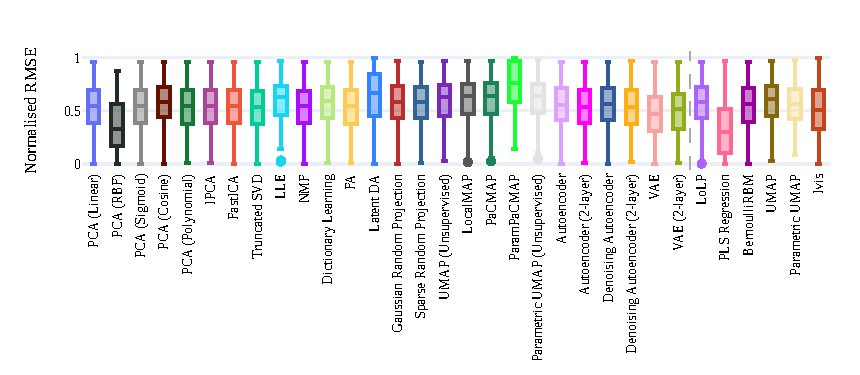
\includegraphics[width=\textwidth]{figures/04/epm/agg_sample_red_inpt_500_1000_40.pdf}
        \caption{\footnotesize$D = 1000, k = 40, N = 500$}
    \end{subfigure}
    \begin{subfigure}[t]{0.24\textwidth}
        \centering
        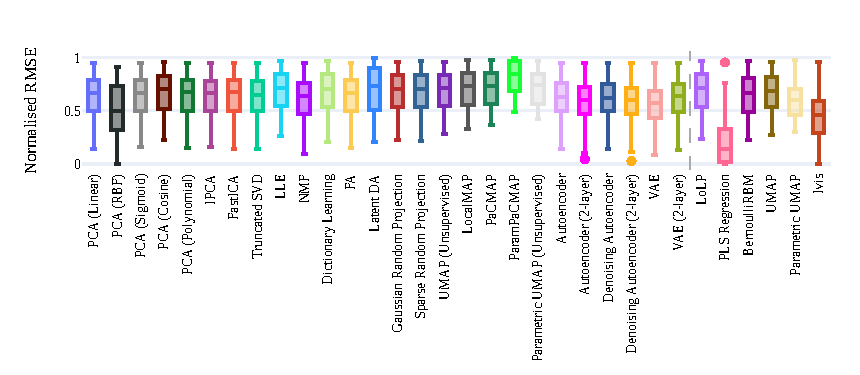
\includegraphics[width=\textwidth]{figures/04/epm/agg_sample_red_inpt_1000_1000_40.pdf}
        \caption{\footnotesize$D = 1000, k = 40, N = 1000$}
    \end{subfigure}
    \hspace{0.2cm}
    \begin{subfigure}[t]{0.8\textwidth}
        \centering
        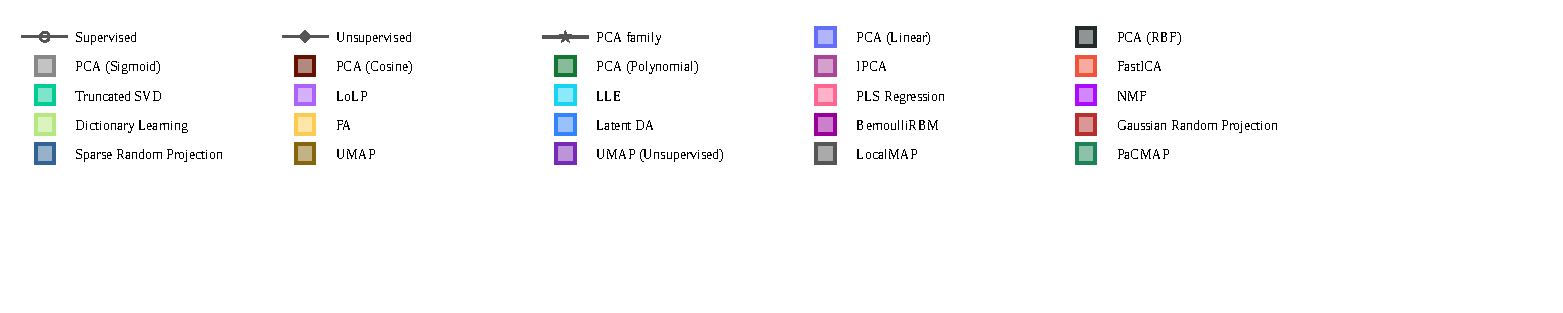
\includegraphics[width=1.0\textwidth,trim={1.5cm 4cm 3.7cm 0.0cm},clip]{figures/04/legend.pdf}
    \end{subfigure}
    \caption[Target function approximation quality by dimensionality]{

    Performance of different dimensionality reduction methods aggregated across synthetic benchmark problems for different initial sample sizes $N$ in two settings: (a-d) with input dimensionality $D = 40$ and target dimensionality $k = 5$, and (e-h) with input dimensionality $D = 1000$ and target dimensionality $k = 40$, in terms of min-max normalised mean \gls{rmse} on \textbf{black-box optimisation task 1: target function approximation}; lower is better.
    Initial sample size has almost no effect when the dimensionality reduction is performed from an already low-dimensional space into an even lower-dimensional one. On the other hand, for a more drastic dimensionality reduction from a very high-dimensional space into a relatively low-dimensional one, a large initial sample size is necessary for accurate target function approximation. 



    }
    \label{fig:ch04:res-bbo-task2_samp_sizes}
\end{figure}


We now analyse the effect of varying initial sample sizes for training dimensionality reduction methods. \cref{fig:ch04:res-bbo-task2_samp_sizes} shows the results aggregated across all different initial sample sizes ($N \in \{100, 200, 500, 1000\}$) for two settings: low-dimensional inputs ($D = 40$, target dimensionality $k = 5$; figures a–d) and high-dimensional inputs ($D = 1000$, target dimensionality $k = 40$; figures e–h).

For the low-dimensional setting ($D = 40$), performance is largely stable across different initial sample sizes. This stability likely arises due to the fact that even the smallest initial sample size already exceeds the number of input dimensions, providing sufficient information for reliable component extraction.
In contrast, for high-dimensional inputs ($D = 1000$), variance decreases noticeably as the initial sample size grows. With $1000$ samples used for dimensionality reduction training, the variance approaches levels observed in the low-dimensional case. This indicates that, although the dimensionality reduction methods are designed to work with limited data, they still depend on sufficient initial sample size (especially when input dimensionality is large) to produce stable and reliable results in predictive tasks.

\begin{figure}
    \centering
    \begin{subfigure}[t]{0.24\textwidth}
        \centering
        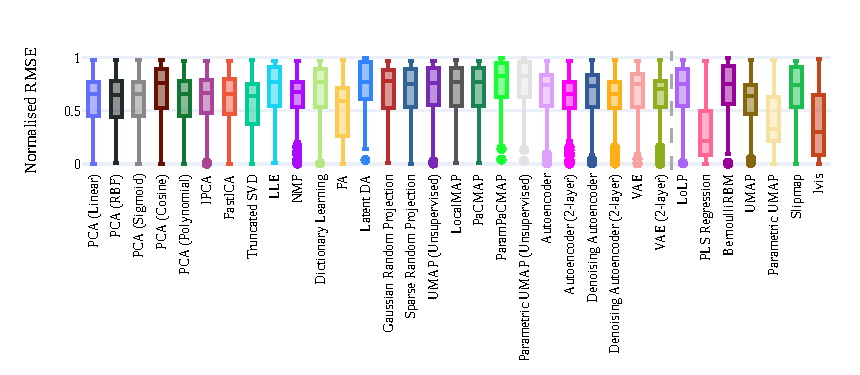
\includegraphics[width=\textwidth]{figures/04/epm/real_agg_sample_red_dim_1000_5.pdf}
        \caption{$N = 100, k=5$}
    \end{subfigure}
    \begin{subfigure}[t]{0.24\textwidth}
        \centering
        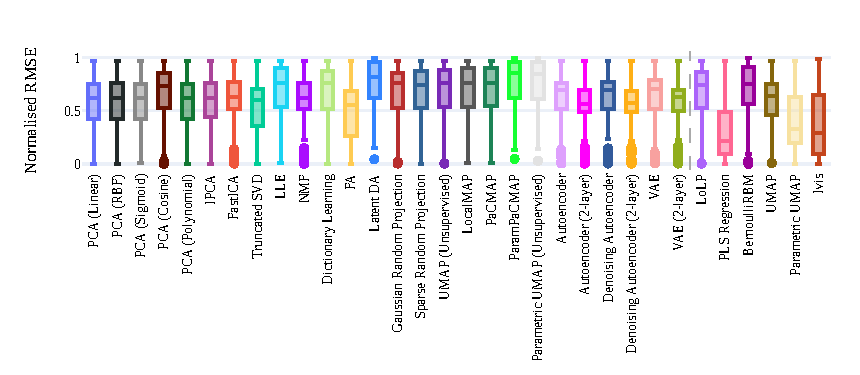
\includegraphics[width=\textwidth]{figures/04/epm/real_agg_sample_red_dim_1000_10.pdf}
        \caption{$N = 100, k=10$}
    \end{subfigure}
    \begin{subfigure}[t]{0.24\textwidth}
        \centering
        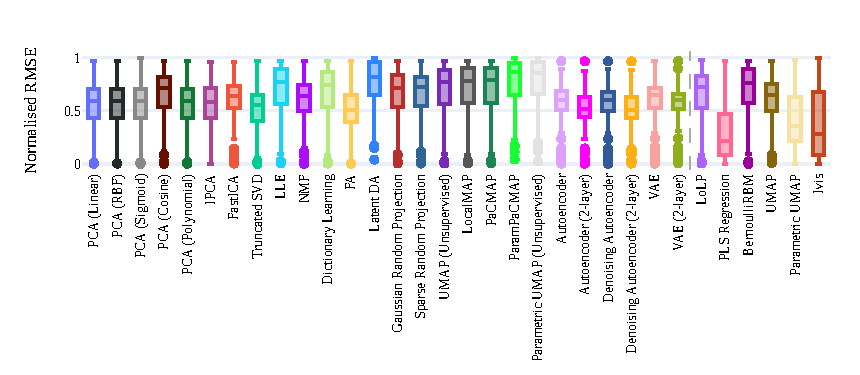
\includegraphics[width=\textwidth]{figures/04/epm/real_agg_sample_red_dim_1000_20.pdf}
        \caption{$N = 100, k=20$}
    \end{subfigure}
    \begin{subfigure}[t]{0.24\textwidth}
        \centering
        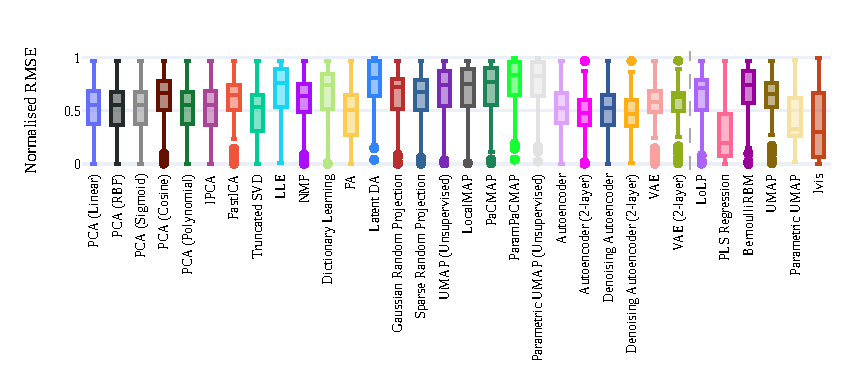
\includegraphics[width=\textwidth]{figures/04/epm/real_agg_sample_red_dim_1000_40.pdf}
        \caption{$N = 100, k=40$}
    \end{subfigure}
    \begin{subfigure}[t]{0.24\textwidth}
        \centering
        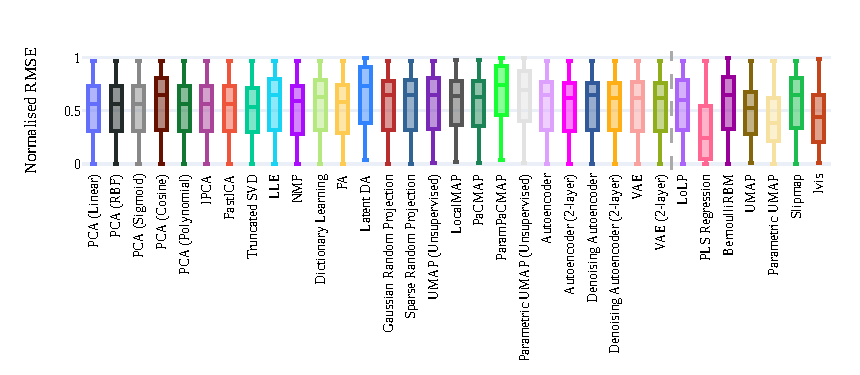
\includegraphics[width=\textwidth]{figures/04/epm/real_agg_sample_red_dim_100_5.pdf}
        \caption{$k = 5, N = 100$}
    \end{subfigure}
    \begin{subfigure}[t]{0.24\textwidth}
        \centering
        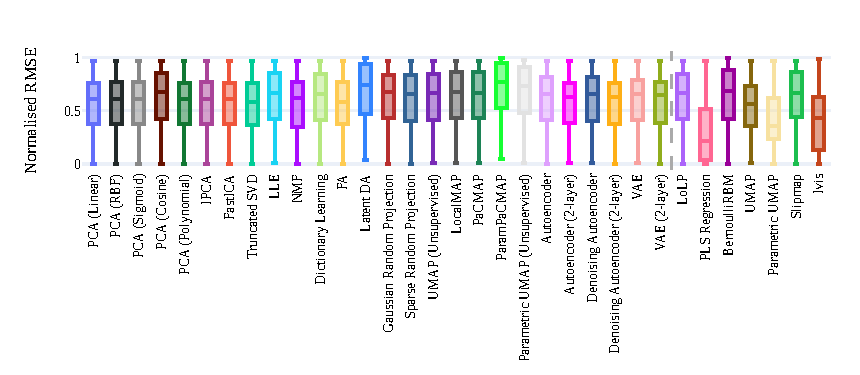
\includegraphics[width=\textwidth]{figures/04/epm/real_agg_sample_red_dim_200_5.pdf}
        \caption{$k = 5, N = 200$}
    \end{subfigure}
    \begin{subfigure}[t]{0.24\textwidth}
        \centering
        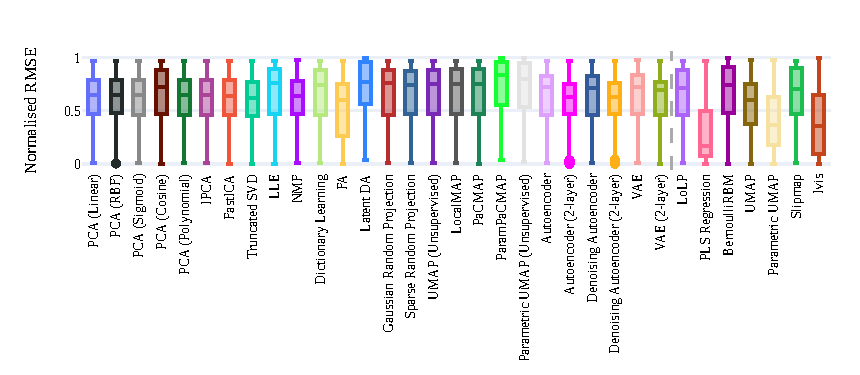
\includegraphics[width=\textwidth]{figures/04/epm/real_agg_sample_red_dim_500_5.pdf}
        \caption{$k = 5, N = 500$}
    \end{subfigure}
    \begin{subfigure}[t]{0.24\textwidth}
        \centering
        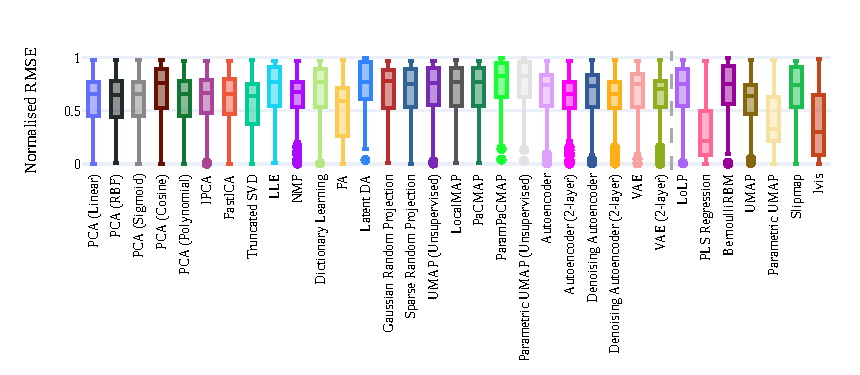
\includegraphics[width=\textwidth]{figures/04/epm/real_agg_sample_red_dim_1000_5.pdf}
        \caption{$k = 5, N = 1000$}
    \end{subfigure}





    \caption[Target function approximation on BBO task 1 for low- and high-dimensional benchmarks]{

    Performance of different dimensionality reduction methods aggregated across real-world benchmark problems in two settings: (a-d) for different target dimensionalities $k$ with initial sample size $N = 100$, and (e-h) for different initial sample sizes $N$ with target dimensionality $k = 5$, in terms of min-max normalised mean \gls{rmse} on \textbf{black-box optimisation task 1: target function approximation}; lower is better.
    Note that the input dimensionality is determined by the benchmark and cannot be controlled.
    PLS regression outperforms other methods across all target dimensionalities even when the initial sample size is small.




    }
    \label{fig:ch04:res-bbo-task1_real}
\end{figure}

So far, our assessment has focused on synthetic benchmarks for black-box optimisation. \cref{fig:ch04:res-bbo-task1_real} shows the results on real-world benchmarks. Figures (a–d) illustrate performance across varying target dimensionalities, with the initial sample size fixed at $N = 100$ (note that input dimensionality is determined by the benchmark and cannot be controlled). Across all target dimensionalities, PLS regression consistently outperforms other methods, reflecting its ability to extract components that are directly predictive of the target variables.
Figures (e–g) show the effect of varying the initial sample size while keeping the target dimensionality fixed at $k = 5$. Similar to the synthetic experiments, performance is relatively comparable across methods at smaller initial sample sizes, likely because most real-world benchmarks are high-dimensional, and small initial sample sizes limit the ability of the methods to extract reliable components. At an initial sample size of $N = 1000$, however, PLS regression clearly emerges as the best-performing method, confirming that adequate initial sample size is crucial for its predictive advantage in real-world, high-dimensional tasks.


\subsubsection*{Black-box optimisation task 2: Optimiser performance}

We now focus on the results of black-box optimisation task 2, where Bayesian optimisation is assisted by the dimensionality reduction methods. As in the previous task, we vary the target dimensionality $k$, while fixing both the initial sample size to $N = 100$ and the original input dimensionality to $D = 120$. The aggregated results across all synthetic benchmark problems are shown in \cref{fig:ch04:res-bbo-task2_red_dim}.
In contrast to the previous black-box optimisation task, PCA (RBF) consistently exhibits best performance across all target dimensionalities. Interestingly, PCA (Cosine) shows a noticeable improvement compared to its performance in the previous task, although it still falls short of PCA (RBF).

In contrast to relatively good performance of LLE in the machine learning task 1 (clustering ability), it is consistently the worst performing method in this task, closely followed by Bernoulli RBM for the highest target dimensionality.



\begin{figure}
    \centering
    \begin{subfigure}[t]{0.24\textwidth}
        \centering
        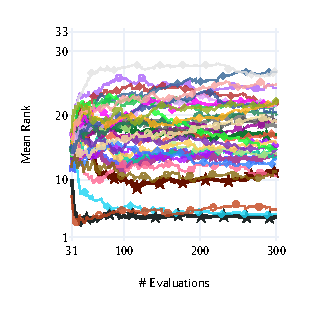
\includegraphics[width=\textwidth]{figures/04/bop/rank_100_120_5.pdf}
        \caption{$k=5$}
    \end{subfigure}
    \begin{subfigure}[t]{0.24\textwidth}
        \centering
        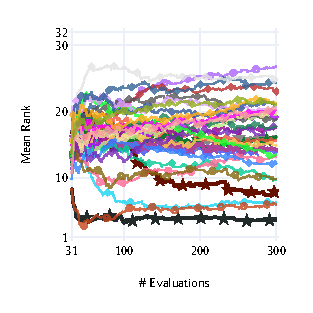
\includegraphics[width=\textwidth]{figures/04/bop/rank_100_120_10.pdf}
        \caption{$k=10$}
    \end{subfigure}
    \begin{subfigure}[t]{0.24\textwidth}
        \centering
        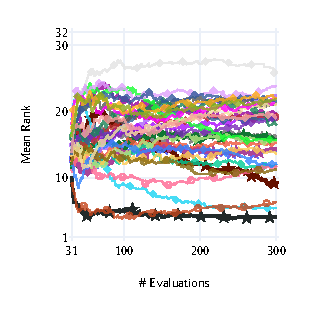
\includegraphics[width=\textwidth]{figures/04/bop/rank_100_120_20.pdf}
        \caption{$k=20$}
    \end{subfigure}
    \begin{subfigure}[t]{0.24\textwidth}
        \centering
        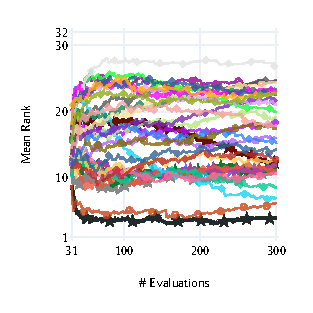
\includegraphics[width=\textwidth]{figures/04/bop/rank_100_120_40.pdf}
        \caption{$k=40$}
    \end{subfigure}
    \begin{subfigure}[t]{0.8\textwidth}
        \centering
        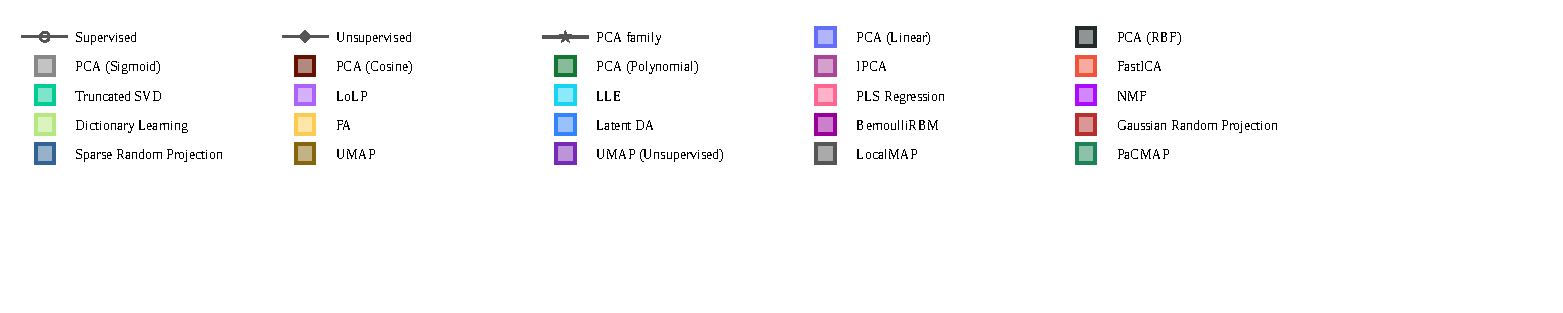
\includegraphics[width=1.0\textwidth,trim={1.5cm 4cm 3.7cm 0.0cm},clip]{figures/04/legend.pdf}
    \end{subfigure}
    \caption[Optimiser performance ranks on BBO task 2]{

    Performance of different dimensionality reduction methods aggregated across synthetic benchmark problems for different target dimensionalities $k$ with input dimensionality $D = 120$ and initial sample size $N = 100$, in terms of mean rank trajectories over the optimisation process on \textbf{black-box optimisation task 2: optimiser performance}; lower rank is better. 
    PCA (RBF) strongly outperforms all other methods across all target dimensionalities, followed by PLS regression and PCA (Cosine) for low target dimensionalities.
    LLE is the worst performing method, followed by Bernoulli RBM in the highest target dimensionality.


    }
    \label{fig:ch04:res-bbo-task2_red_dim}
\end{figure}

Next, we analyse the effect of varying input dimensionalities $D$ while fixing the initial sample size at $N = 100$ and the target dimensionality at $k = 20$.~\cref{fig:ch04:res-bbo-task2_diff_dims} shows the results aggregated across all synthetic benchmark problems. Across all input dimensionalities, PCA (RBF) consistently outperforms the other methods, confirming its robustness in this task.
Interestingly, unlike in black-box optimisation task 1 (target function approximation, which can also be seen as performance prediction from the point of view of empirical performance models~\citep{HutEtAl14}), where PLS regression excelled at lower input dimensionalities, here it performs better on higher-dimensional inputs on average. This shift likely reflects the difference in task objectives: in Bayesian optimisation, capturing broader input-space structure becomes more important as dimensionality increases, allowing PLS regression to extract useful predictive directions even without low-dimensional constraints.
Additionally, PCA (Cosine) shows improved performance across all input dimensionalities compared to the previous task, though it still remains slightly below PCA (RBF), suggesting that kernel-based PCA variants generally benefit more from the unsupervised optimisation setting.

Last, LLE exhibits consistent poor performance, in line with the previous findings for this task.


\begin{figure}
    \begin{subfigure}[t]{0.32\textwidth}
        \centering
        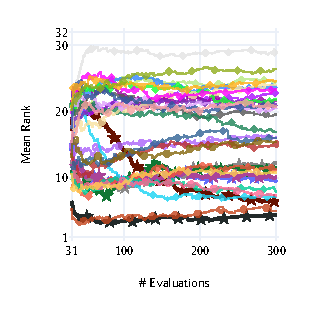
\includegraphics[width=\textwidth]{figures/04/bop/rank_100_40_20.pdf}
        \caption{$D=40$}
    \end{subfigure}
    \begin{subfigure}[t]{0.32\textwidth}
        \centering
        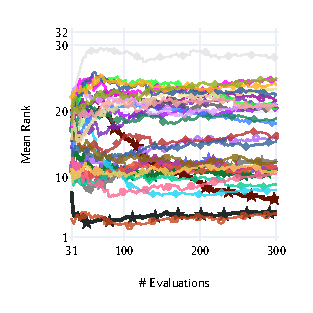
\includegraphics[width=\textwidth]{figures/04/bop/rank_100_60_20.pdf}
        \caption{$D=60$}
    \end{subfigure}
    \begin{subfigure}[t]{0.32\textwidth}
        \centering
        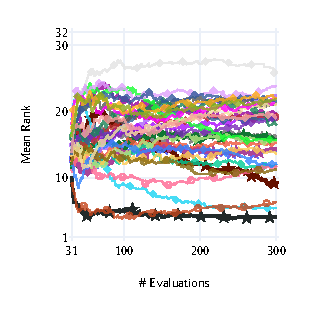
\includegraphics[width=\textwidth]{figures/04/bop/rank_100_120_20.pdf}
        \caption{$D=120$}
    \end{subfigure}
    \begin{subfigure}[t]{0.32\textwidth}
        \centering
        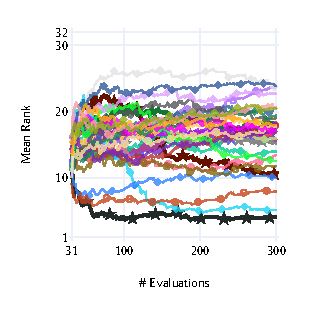
\includegraphics[width=\textwidth]{figures/04/bop/rank_100_240_20.pdf}
        \caption{$D=240$}
    \end{subfigure}
    \begin{subfigure}[t]{0.32\textwidth}
        \centering
        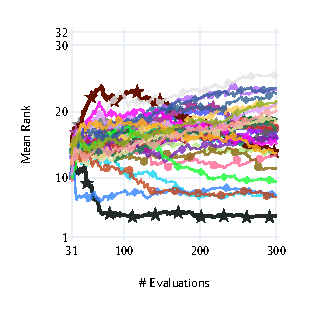
\includegraphics[width=\textwidth]{figures/04/bop/rank_100_500_20.pdf}
        \caption{$D=500$}
    \end{subfigure}
    \begin{subfigure}[t]{0.32\textwidth}
        \centering
        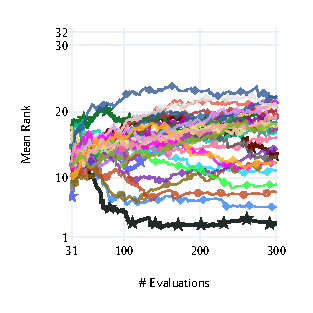
\includegraphics[width=\textwidth]{figures/04/bop/rank_100_1000_20.pdf}
        \caption{$D=1000$}
    \end{subfigure}
    \hspace{0.2cm}
    \begin{subfigure}[t]{0.8\textwidth}
        \centering
        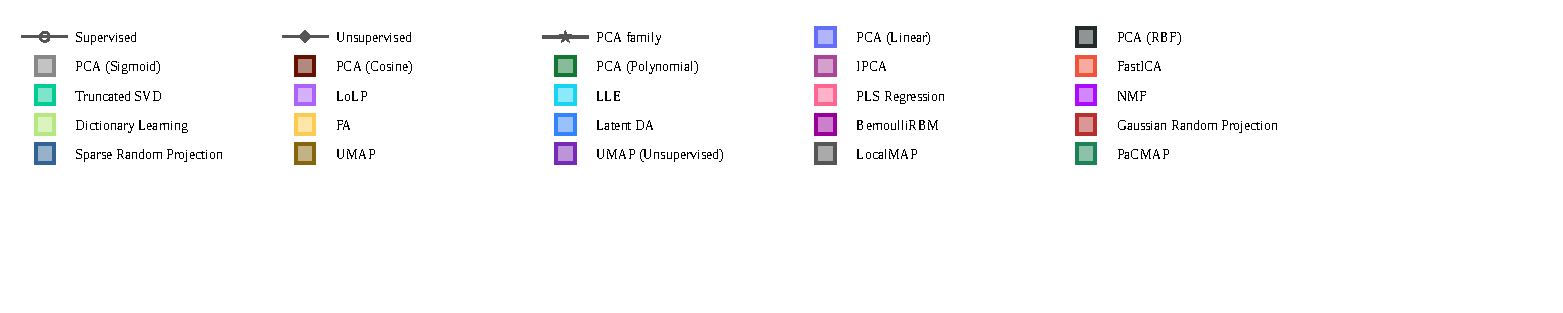
\includegraphics[width=1.0\textwidth,trim={1.5cm 4cm 3.7cm 0.0cm},clip]{figures/04/legend.pdf}
    \end{subfigure}
    \caption[Optimiser performance ranks on BBO task 2 by dimensionality]{

    Performance of different dimensionality reduction methods aggregated across synthetic benchmark problems for different input dimensionalities $D$ with target dimensionality $k = 20$ and initial sample size $N = 100$, in terms of mean rank trajectories over the optimisation process on \textbf{black-box optimisation task 2: optimiser performance}; lower rank is better. 
    PCA (RBF) strongly dominates all other methods across all input dimensionalities, followed by PLS regression for high input dimensionalities.
    PCA (Cosine) rapidly catches up with the top-ranked methods for lower-dimensional inputs, outranking PLS regression for $D = 240$ in the last stage of the optimisation process, but still consistently failing to outperform PCA (RBF).
    LLE is the worst performing method, followed by dictionary learning and Bernoulli RBM for lower input dimensionalities.


    }
    \label{fig:ch04:res-bbo-task2_diff_dims}
\end{figure}

We further examine the effect of varying initial sample sizes $N$ on performance, as shown in \cref{fig:ch04:res-bbo-task2_samples}. Figures (a–d) correspond to low-dimensional inputs ($D = 40$) with target dimensionality fixed at $k = 5$. In this setting, PCA (RBF) generally performs best, although PCA (Cosine) competes closely at small initial sample sizes, suggesting that with limited data, the choice of kernel can influence the stability of the projection.
Figures (e–h) show the results for high-dimensional inputs ($D = 1000$) with target dimensionality fixed at $k = 40$. Here, PLS regression performs comparably to PCA (RBF) when the initial sample size is large, indicating that with sufficient data, supervised methods can extract predictive directions even in very high-dimensional spaces, narrowing the gap with unsupervised methods.
\begin{figure}
    \centering
    \begin{subfigure}[t]{0.24\textwidth}
        \centering
        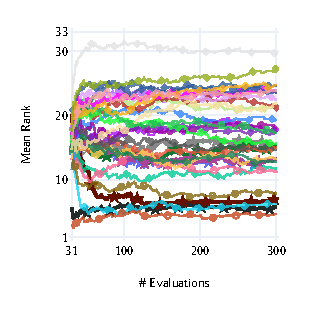
\includegraphics[width=\textwidth]{figures/04/bop/rank_100_40_5.pdf}
        \caption{\footnotesize$D = 40, k = 5, N = 100$}
    \end{subfigure}
    \begin{subfigure}[t]{0.24\textwidth}
        \centering
        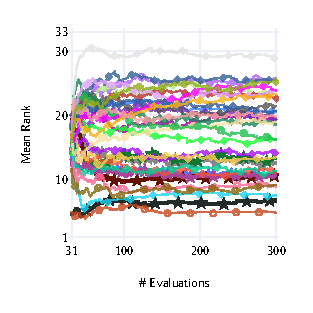
\includegraphics[width=\textwidth]{figures/04/bop/rank_200_40_5.pdf}
        \caption{\footnotesize$D = 40, k = 5, N = 200$}
    \end{subfigure}
    \begin{subfigure}[t]{0.24\textwidth}
        \centering
        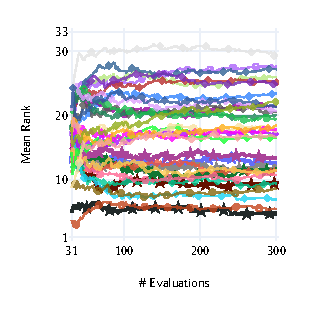
\includegraphics[width=\textwidth]{figures/04/bop/rank_500_40_5.pdf}
        \caption{\footnotesize$D = 40, k = 5, N = 500$}
    \end{subfigure}
    \begin{subfigure}[t]{0.24\textwidth}
        \centering
        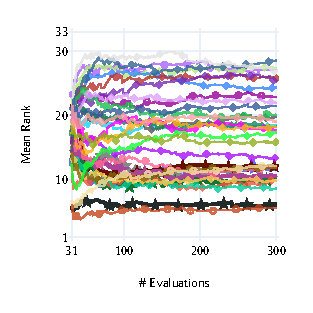
\includegraphics[width=\textwidth]{figures/04/bop/rank_1000_40_5.pdf}
        \caption{\footnotesize$D = 40, k = 5, N = 1000$}
    \end{subfigure}
    \begin{subfigure}[t]{0.24\textwidth}
        \centering
        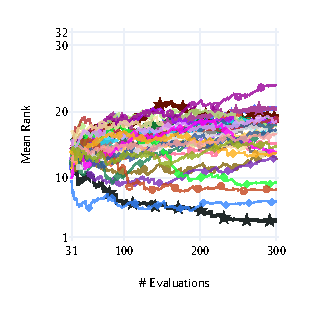
\includegraphics[width=\textwidth]{figures/04/bop/rank_100_1000_40.pdf}
        \caption{\footnotesize$D = 1000, k = 40, N = 100$}
    \end{subfigure}
    \begin{subfigure}[t]{0.24\textwidth}
        \centering
        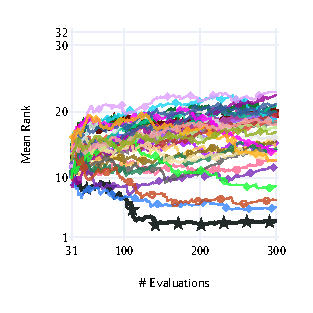
\includegraphics[width=\textwidth]{figures/04/bop/rank_200_1000_40.pdf}
        \caption{\footnotesize$D = 1000, k = 40, N = 200$}
    \end{subfigure}
    \begin{subfigure}[t]{0.24\textwidth}
        \centering
        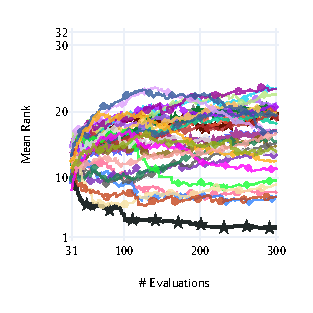
\includegraphics[width=\textwidth]{figures/04/bop/rank_500_1000_40.pdf}
        \caption{\footnotesize$D = 1000, k = 40, N = 500$}
    \end{subfigure}
    \begin{subfigure}[t]{0.24\textwidth}
        \centering
        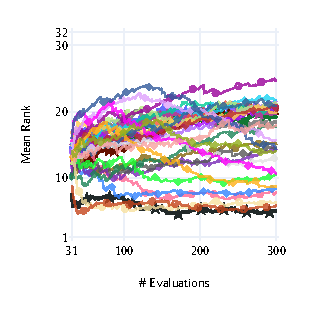
\includegraphics[width=\textwidth]{figures/04/bop/rank_1000_1000_40.pdf}
        \caption{\footnotesize$D = 1000, k = 40, N = 1000$}
    \end{subfigure}
    \hspace{0.2cm}
    \begin{subfigure}[t]{0.8\textwidth}
        \centering
        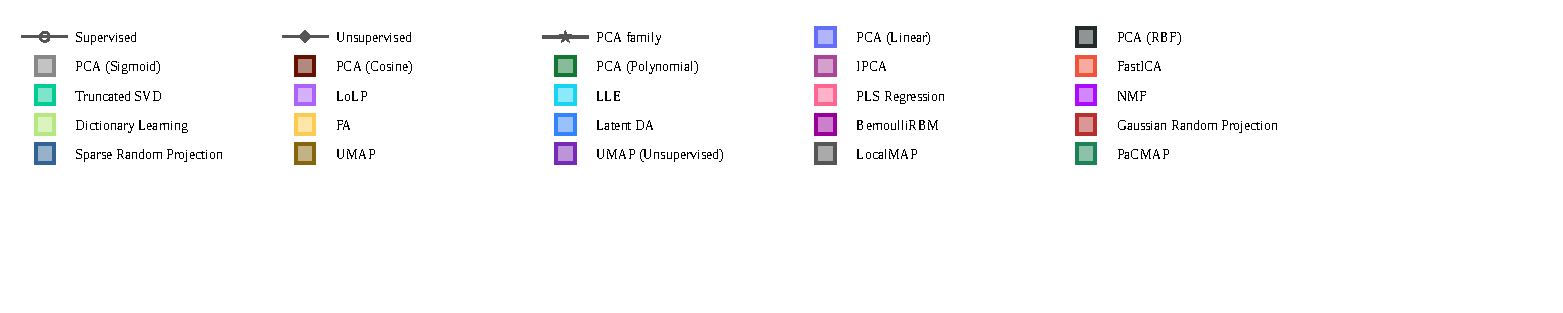
\includegraphics[width=1.0\textwidth,trim={1.5cm 4cm 3.7cm 0.0cm},clip]{figures/04/legend.pdf}
    \end{subfigure}
    \caption[Optimiser performance ranks on BBO task 2 for low- and high-dimensional benchmarks]{

    Performance of different dimensionality reduction methods aggregated across synthetic benchmark problems for different initial sample sizes $N$ in two settings: (a-d) with input dimensionality $D = 40$ and target dimensionality $k = 5$, and (e-h) with input dimensionality $D = 1000$ and target dimensionality $k = 40$, in terms of mean rank trajectories over the optimisation process on \textbf{black-box optimisation task 2: optimiser performance}; lower rank is better.
    PCA (RBF) is the top-ranked method across both settings, while PLS regression exhibits stronger performance for high-dimensional inputs than for low-dimensional ones.
    Dictionary learning, LLE, Bernoulli RBM and PCA (Cosine) are among the worst performers for low-dimensional inputs, whereas for high input dimensionalities, LLE stands out with its poor performance when the initial sample size is low, but quickly becomes indistinguishable from, \emph{e.g.,}, Bernoulli RBM (and other methods) as the initial sample size increases.


    }
    \label{fig:ch04:res-bbo-task2_samples}
\end{figure}


Finally, we look into the results on real-world benchmark problems in~\cref{fig:ch04:res-bbo-task2-real-world}, which paint a considerably different picture than synthetic benchmarks.
In Figures (a-d) we investigate the impact of varying target dimensionality $k$ while keeping the initial sample size fixed at $N = 100$. 
Unlike synthetic benchmarks where higher value of target dimensionality allowed for a relatively consistent performance improvement, here we see more complex optimisation dynamics, with highly variable performance across methods.
At the lowest target dimensionality we observe the most diverse performance of all methods, and the rapid convergence followed by plateaus suggests that most of the intrinsic information in dimension $5$ is captured early on in the optimisation process.
When target dimensionality is increased from $k = 20$ to $k = 40$, performance does not drastically improve, even though the advantage of methods that exhibited good performance for low values of $k$ diminishes.
This suggests that real-world optimisation problems may have intrinsic dimensionality in the range of $10$ to $20$ dimensions that are effectively exploitable (even with a small initial sample size of $100$), while additional target dimensions yield limited benefit and can even make the optimisation process more challenging.
Notably, for different target dimensionalities we cannot distinguish a clear winner among dimensionality reduction methods, while LLE is especially ill-suited for higher values of $k$ on this task.

Last, we assess the impact of varying initial sample sizes $N$ while keeping the target dimensionality fixed at $k = 5$ in Figures (e-h). 
Most methods start off with strong fluctuations in their convergence curves at the smallest initial sample size, suggesting that an insufficient amount of training data leads to unreliable dimensionality reduction mapping.
As the initial sample size increases, the convergence curves become smoother and more regular, and the performance gap between two distinct sets of methods becomes apparent.
Among good performers, we find in particular all PCA variants (with a notable exception of PCA (Cosine)), and PLS regression (which is top-ranked for the initial sample size of $N = 200$, and showed a consistent strong performance in the previous black-box optimisation task, as well as in this task on synthetic benchmarks).
Poor performance was yielded by LLE, Bernoulli RBM, LoLP, Gaussian and sparse random projections, dictionary learning, and, surprisingly, PCA (Cosine), which was often among the three top-ranked dimensionality reduction methods on synthetic benchmarks in this task.
The results indicate that the initial sample size used for training dimensionality reduction methods critically affects both optimisation quality and smoothness of convergence in real-world scenarios.
Moreover, as real-world function evaluations are expensive, this highlights a trade-off in allocating evaluations for training dimensionality reduction methods and for running the optimiser itself.

Overall, stark differences between performances of the methods on synthetic vs. real-world benchmarks likely reflect the heterogeneous nature of real-world problems, where features defining the search space often come from various domains and have complex interactions.
Across almost all considered settings, there is an evident tendency for methods to plateau well before the full optimisation budget is exhausted, causing the performance to stagnate.
This might indicate that, on real-world problems, the optimiser assisted by dimensionality reduction can effectively exploit only the global structure preserved in the reduced space, but loses access to more fine-grained details of these complex landscapes.
Finally, through high variability of observed behaviours across all settings, we see a general pattern of performance complementarity of different dimensionality reduction methods; while some methods excel on some problems, they perform poorly on others. 






\begin{figure}
    \centering
    \begin{subfigure}[t]{0.24\textwidth}
        \centering
        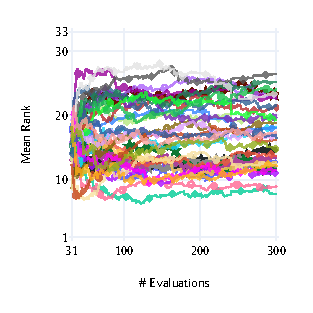
\includegraphics[width=\textwidth]{figures/04/bop/rank_real_100_5.pdf}
        \caption{$N = 100, k = 5$}
    \end{subfigure}
    \begin{subfigure}[t]{0.24\textwidth}
        \centering
        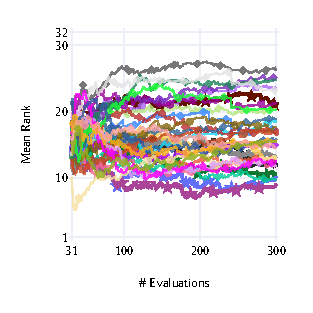
\includegraphics[width=\textwidth]{figures/04/bop/rank_real_100_10.pdf}
        \caption{$N = 100, k = 10$}
    \end{subfigure}
    \begin{subfigure}[t]{0.24\textwidth}
        \centering
        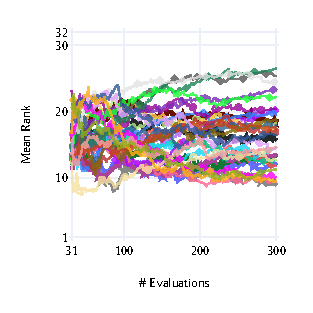
\includegraphics[width=\textwidth]{figures/04/bop/rank_real_100_20.pdf}
        \caption{$N = 100, k = 20$}
    \end{subfigure}
    \begin{subfigure}[t]{0.24\textwidth}
        \centering
        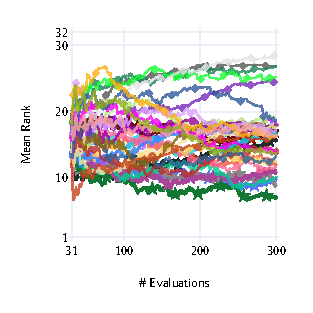
\includegraphics[width=\textwidth]{figures/04/bop/rank_real_100_40.pdf}
        \caption{$N = 100, k = 40$}
    \end{subfigure}
    \begin{subfigure}[t]{0.24\textwidth}
        \centering
        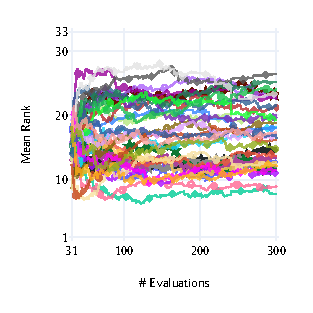
\includegraphics[width=\textwidth]{figures/04/bop/rank_real_100_5.pdf}
        \caption{$k = 5, N = 100$}
    \end{subfigure}
    \begin{subfigure}[t]{0.24\textwidth}
        \centering
        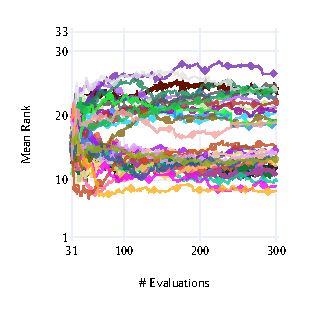
\includegraphics[width=\textwidth]{figures/04/bop/rank_real_200_5.pdf}
        \caption{$k = 5, N = 200$}
    \end{subfigure}
    \begin{subfigure}[t]{0.24\textwidth}
        \centering
        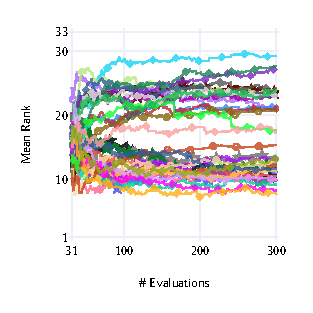
\includegraphics[width=\textwidth]{figures/04/bop/rank_real_500_5.pdf}
        \caption{$k = 5, N = 500$}
    \end{subfigure}
    \begin{subfigure}[t]{0.24\textwidth}
        \centering
        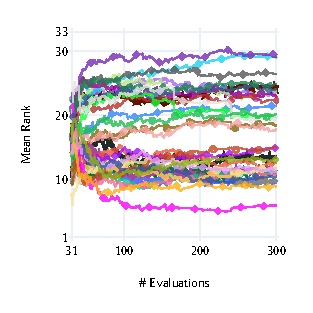
\includegraphics[width=\textwidth]{figures/04/bop/rank_real_1000_5.pdf}
        \caption{$k = 5, N = 1000$}
    \end{subfigure}
    \hspace{0.2cm}
    \begin{subfigure}[t]{0.8\textwidth}
        \centering
        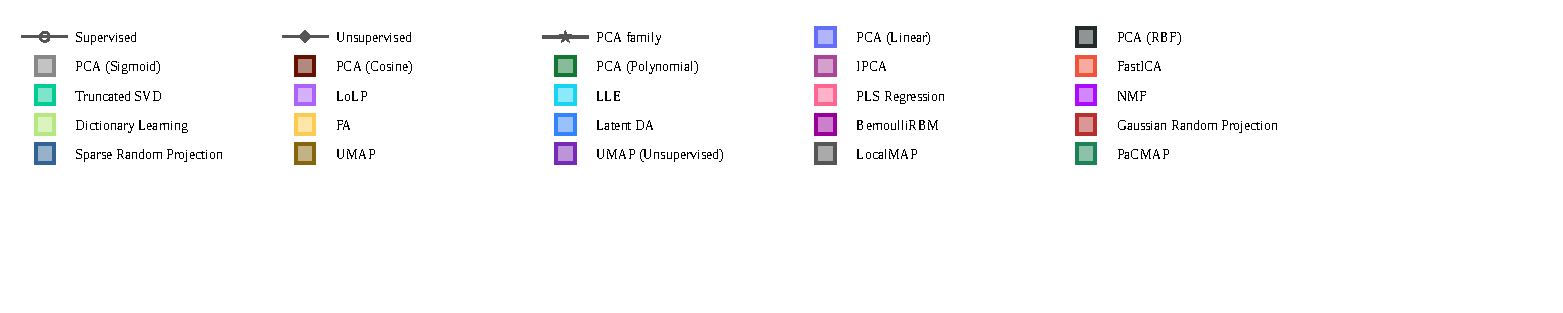
\includegraphics[width=1.0\textwidth,trim={1.5cm 4cm 3.7cm 0.0cm},clip]{figures/04/legend.pdf}
    \end{subfigure}
    \caption[Optimiser performance ranks on BBO task 2 for real-world benchmarks]{

    Performance of different dimensionality reduction methods aggregated across real-world benchmark problems in two settings: (a-d) for different target dimensionalities $k$ with initial sample size $N = 100$, and (e-h) for different initial sample sizes $N$ with target dimensionality $k = 5$, in terms of mean rank trajectories over the optimisation process on \textbf{black-box optimisation task 2: optimiser performance}; lower rank is better. Note that (i) the input dimensionality is determined by the benchmark and cannot be controlled, and (ii) figures (a) and (e) correspond to the same scenario.
    In the first setting, there is no single top-ranked method; LLE stands out as the worst performing method for higher target dimensionalities.
    In the second setting, as the number of initial samples grows, there appears a substantial spread in performance between two distinct sets of methods; notably, PCA (Cosine) is among the worst performers.


    }
    \label{fig:ch04:res-bbo-task2-real-world}
\end{figure}


\section{Running times}
\label{sec:ch04:rt}


In~\cref{fig:ch04:res-rt} we present the training and transformation running times of the dimensionality reduction methods for 2 selected OpenML datasets 

used in machine learning tasks 1 and 2: one with a lower dimensionality and a high number of elements, and one with a higher dimensionality and a low number of elements.

The running times are reported as CPU time.
We note that we report the transformation time 

needed for the two machine learning tasks,

but the times for black-box optimisation task 1 are similar 
as in this task we simply train and transform on a fixed dataset.

For black-box optimisation task 2, it is 

more challenging to isolate

the effect of the running time of the dimensionality reduction itself, as it is 

integrated in
the surrogate training and acquisition function optimisation, which are additional factors that can greatly affect the total running time.

We observe that for both training and transformation of low-dimensional datasets with a high number of elements (Figures (a-b)), LLE and PCA variants with non-linear kernels exhibit the highest running times.

For the high-dimensional dataset with a low number of elements (Figures (c-d)), the running times of those methods is lower compared to most other methods. In this setting, dictionary learning is the most expensive method in terms of running time.

We observe that Gaussian and sparse random projections consistently incur low running times, and that PLS regression is quite competitive in this regard for both datasets.



\begin{figure}
    \centering
    \begin{subfigure}[t]{0.24\textwidth}
        \centering
        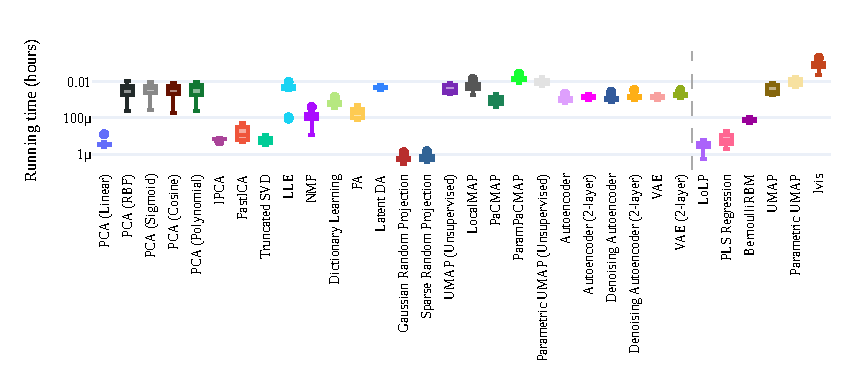
\includegraphics[width=\textwidth]{figures/04/time/9985_train_time.pdf}
        \caption{Training on dataset 9985}
    \end{subfigure}
    \begin{subfigure}[t]{0.24\textwidth}
        \centering
        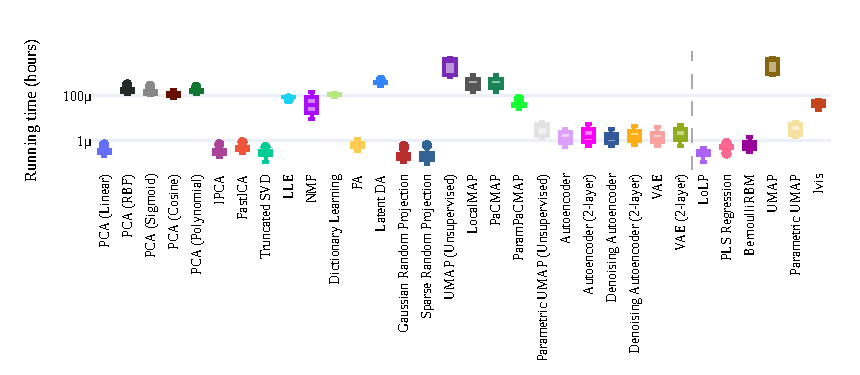
\includegraphics[width=\textwidth]{figures/04/time/9985_transform_time.pdf}
        \caption{Transform on dataset 9985}
    \end{subfigure}
        \begin{subfigure}[t]{0.24\textwidth}
        \centering
        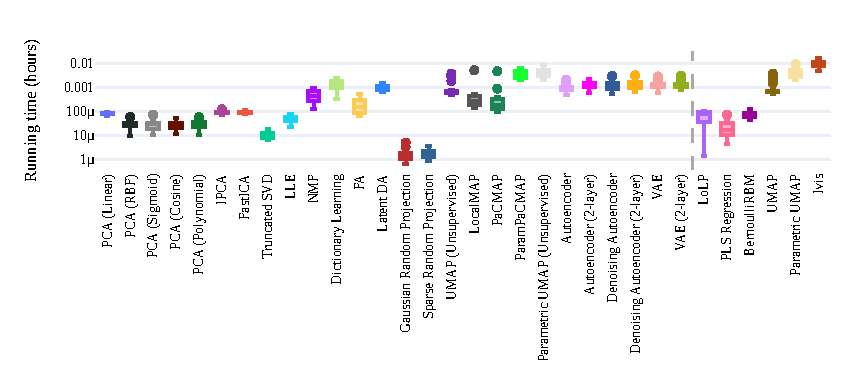
\includegraphics[width=\textwidth]{figures/04/time/9981_train_time.pdf}
        \caption{Train on dataset 9981}
    \end{subfigure}
    \begin{subfigure}[t]{0.24\textwidth}
        \centering
        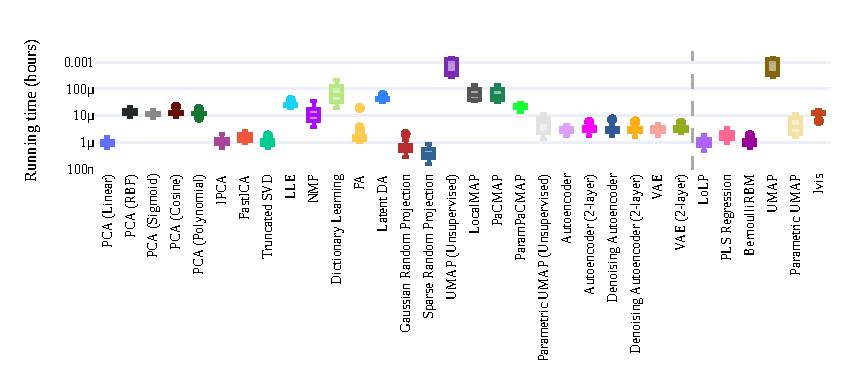
\includegraphics[width=\textwidth]{figures/04/time/9981_transform_time.pdf}
        \caption{Transform on dataset 9981}
    \end{subfigure}
    \caption[CPU hours for training and transformation]{

    Running times in terms of CPU hours for dimensionality reduction training (a, c) and transformation (b, d) of OpenML datasets 9985 (51 features and 6618 elements) and 9981 (856 features and 1080 elements).

    }
    \label{fig:ch04:res-rt}
\end{figure}



\section{Discussion}
\label{sec:ch04:disc}


Our comprehensive assessment of dimensionality reduction methods reveals fundamental differences in how the benchmarked methods perform in machine learning and black-box optimisation contexts.
An important insight of this study is the existence of strong task-dependent performance complementarity, as no single dimensionality reduction method dominates across all tasks.
This observation underscores that, to achieve best possible performance, proper method selection must be task-driven.

In the machine learning domain, we observed relatively similar performance of most dimensionality reduction methods.
For clustering, most methods struggled to preserve cluster homogeneity, indicating that class boundaries are challenging to capture, while cluster completeness was successfully retained by random projection methods and LLE in higher-dimensional subspaces.
In particular, good performance of LLE in this context may be due to its unsupervised nature and the fact it is designed to capture local structure.
Interestingly, this very characteristic of LLE might be responsible for its poor performance in assisting an optimiser.
For classification, most methods achieved a consistently high accuracy regardless of the underlying machine learning model (with the exception of random projections and Bernoulli RBM), suggesting that for well-structured tabular data, the choice of dimensionality reduction method has limited impact on downstream classification performance.
Both machine learning tasks showed that performance improves monotonically with target dimensionality, meaning that higher-dimensional projections retain more task-relevant information for structured datasets.

On the other hand, in the black-box optimisation domain, the choice of dimensionality reduction method had a substantial impact on the downstream performance, due to strong performance differences between methods.
For target function approximation, PLS regression was a top performer at lower target dimensionalities and moderate input dimensionalities, in line with the fact that it is a supervised method designed with the objective of extracting components directly predictive of function values.
However, for very-high dimensional inputs, or for insufficient data for training dimensionality reduction methods, PCA with the RBF kernel overtook PLS regression as the top-performing method.
A reason for this might be that unsupervised variance-based methods supported by an adequate non-linear kernel are able to capture essential problem structure when the original search space is extremely large and/or not well covered.


For optimiser performance, PCA with the RBF kernel excels by a large margin in assisting Bayesian optimisation in high-dimensional spaces.
This indicates that, in order to successfully perform Bayesian optimisation in the reduced space, dimensionality reduction has to be done via methods that preserve the global geometric structure of the objective function, and not merely predictive components.
For instance, LLE consistently performed worst in this task, showing that preserving local (instead of global) structure is detrimental for assisting optimisation procedures.


In particular, PLS regression (which was top-ranked for target function approximation) is not able to outperform PCA with the RBF kernel here.
Intuitively, this is because accurate prediction of function values does not necessarily translate to effective (and efficient) optimisation, as already observed in~\citep{FeuEtAl18b}.
In other words, problem characteristics required for guiding the search process fundamentally differ from those allowing for accurate function value regression, and the strong performance of PCA with the RBF kernel specifically suggests that capturing non-linear, distance-based relationships in the search space is crucial for optimisation, more so than explicit supervision on objective values.

We note that different sample sizes for training dimensionality reduction methods were used for the two black-box optimisation tasks.
However, as target function approximation via a surrogate model is a key component of Bayesian optimisation, we conjecture that some methods would tend to be effective in enhancing the optimiser, even if the surrogate (in the Bayesian optimisation loop of black-box optimisation task 2) is fitted on a smaller sample than for target function approximation of  black-box optimisation task 1.
We believe these observations to be of great importance for designing out-of-the-box robust Bayesian optimisation-based approaches to tackle high-dimensional real-world problems.















Taken together, these findings suggest that the task objective strongly shapes which dimensionality reduction method is most effective: supervised tasks favour methods aligned with predictive power, while unsupervised tasks benefit from methods that preserve geometric or topological structure.










\section{Chapter conclusion}
\label{sec:ch04:concl}



This chapter assessed the performance of a broad range of dimensionality reduction methods based on four carefully chosen downstream tasks from two different fields: machine learning and black-box optimisation.
Each task allows for empirically evaluating different aspects of dimensionality reduction methods, highlighting the task-dependent differences in their performance.
Specifically, we conducted a thorough benchmarking study of 16 dimensionality reduction methods 

(based on feature extraction) 
on these four tasks across a range of different settings (\emph{i.e.,} original dimensionality, target dimensionality, budget available for training dimensionality reduction methods), 

and derived practical insights into their suitability depending on their intended use.







In general, 

we observed that the choice of dimensionality reduction method depends on the task, as for each of the four tasks, different methods perform best. 

Moreover, even within the same task, different methods work best for different datasets or functions. 

While the performance differences are more prominent in  black-box optimisation tasks than in machine learning ones,

this shows that there is \textit{performance complementarity}~\cite{Rice76,FreEtAl16} between the dimensionality reduction methods, and that careful method selection is of key importance for achieving optimal performance.
In practice, dimensionality reduction methods are typically chosen based on good performance in similar scenarios.

We expect that meta-learning which method to use in which case can yield substantial performance gains and intend to further pursue research in this direction in future work.








Overall, dimensionality reduction methods often play a crucial role for solving problems in high-dimensional spaces. 
The results produced new insights into how these methods work in four broadly interesting scenarios, thus facilitating better understanding of their strengths and weaknesses.
These insights can be used in the future to help design new and improve existing dimensionality reduction methods for specific tasks.

\paragraph{Connection to the thesis}~
The results of this chapter show that there is no universally best representation: the usefulness of a reduced space depends on the downstream task and the structure of the problem.
This naturally leads to the question of how empirical performance prediction methods can adapt when different modelling choices are useful in different situations.
The next chapter addresses this question in Bayesian optimisation by dynamically combining complementary surrogate models.
